\documentclass[../main.tex]{subfiles}
\graphicspath{{\subfix{..}}}
\begin{document}
\chapter{Dualcalorimetric analysis for Precision Measurement}
\label{sec:joint_fit}

\epigraph{``We demand rigidly defined areas of doubt and uncertainty!''}{Douglas Adams, The Hitchhiker’s Guide to the Galaxy}

\minitoc

% I)  Introduction globale.
% -------------------------------------
% ... Aborder les points suivants de manière succinte, pour donner une vision d'ensemble...
%
%     + JUNO est une expérience de physique de précision : il sera indispensable de comprendre très précisément les effets de reconstruction. C'est  d'autant  plus un défi que Juno emploie une technologie standard en physique des neutrinos (sphère ou cuve de scintillateur liquide  + PMT) mais l'amène dans une configuration extrême et inédite (très gros volume de scintillation, PMT de 30 pouces, etc...) où comprendre les effets de détection peut s'avérer difficile. Il est possible de rater quelque chose. Pouvoir comparer les données et résultats issus de deux systèmes indépendants, soumis à des problèmes différents, est donc précieux. C'est l'origine du dev de sPMT en plus des LPMT.
%
%     + L'importance cruciale de la maîtrise de la reconstruction : résolution à mieux que 3% et biais très inférieur à 1% sur la connaissance de la non linéarité sous peine d'incapacité à mesurer la NMO.
% Rappeler cet élément majeur : si on se trompe de 1%, on conclut à la mauvaise NMO. Utiliser la figure donnée dans la thèse de Yang pour appuyer ce point.
%
%    + Une source possible de non linéarité difficile à détecter à ce stade est la QNL. (Voir section suivante pour définition complète).
%
%     + La DC répond à cela. Elle interviendra notamment en fournissant des méthodes de calibration permettant de corriger la QNL. Ne pas en dire plus, ref these Yang.
%
%     + Plus generalement : Comparer deux systèmes pour détecter des problèmes sur la calibration ou la reco de l'un des deux. C'est ce que l'on fait dans cette thèse en comparant directement les résultats de la mesure des params d'oscillation.
%
%    + Une difficulté à étudier : la corrélation entre les deux systèmes : pas suffisant de comparer l'écart entre les valeurs centrales aux incertitudes individuelles. Nous proposons dans ce chapitre une exploration préliminaire testant différentes méthodes, en prédisant la sensibilité de ces méthodes à la présence QNL à divers degrés.
%
%   + Plan du chapitre.

JUNO is precision measurement experiment.
To determine the NMO with the aimed significance, JUNO must be sensitive to the tiny spectral phase shift shown on figure \ref{fig:joint_fit:juno-spectrum-oscillation}.
Once detection effects are accounted for, the difference between IO and NO spectra is further reduced, as can be seen on figure \ref{fig:joint_fit:juno-ordering}.

Among other condition, a precise and complete understanding of the reconstruction and detector effects is crucial.
The challenge reside in the technology used in the detector, which, while based on well known technology: scintillator observed by PMT, is being deployed on a scale never seen before, in term of scintillator volume and  PMT size. Understanding every effects that goes in the detector can become extremely complicated. Any method to help detecting problems is therefore welcome.
Comparing the data and results obtained by two systems measuring the same events, but subject to different sources of error, is therefore precious. This is the purpose of the dual calorimetry techniques used in JUNO thanks to the existence of 2 PMT systems: the LPMT and SPMT systems.

The reconstruction of the IBD positron energy must be very performant: an unprecedented resolution of 3\% at 1 MeV \cite{juno_collaboration_juno_2022} is necessary to determine the NMO with the aimed significance.
Moreover, it is necessary to know the energy scale with an uncertainty below 1\% to correctly evaluate in our data the likelihood of the NO and IO  hypotheses. Beyond that value, the risk progressively appears to exclude the NI(IO) hypothesis with the significance with which  one should actually have excluded the IO(NO) if the energy scale was precisely known, as can be seen in the introduction of Chapter 4 of \cite{han_dual_2021}.

\begin{figure}[ht]
\centering
  \centering
  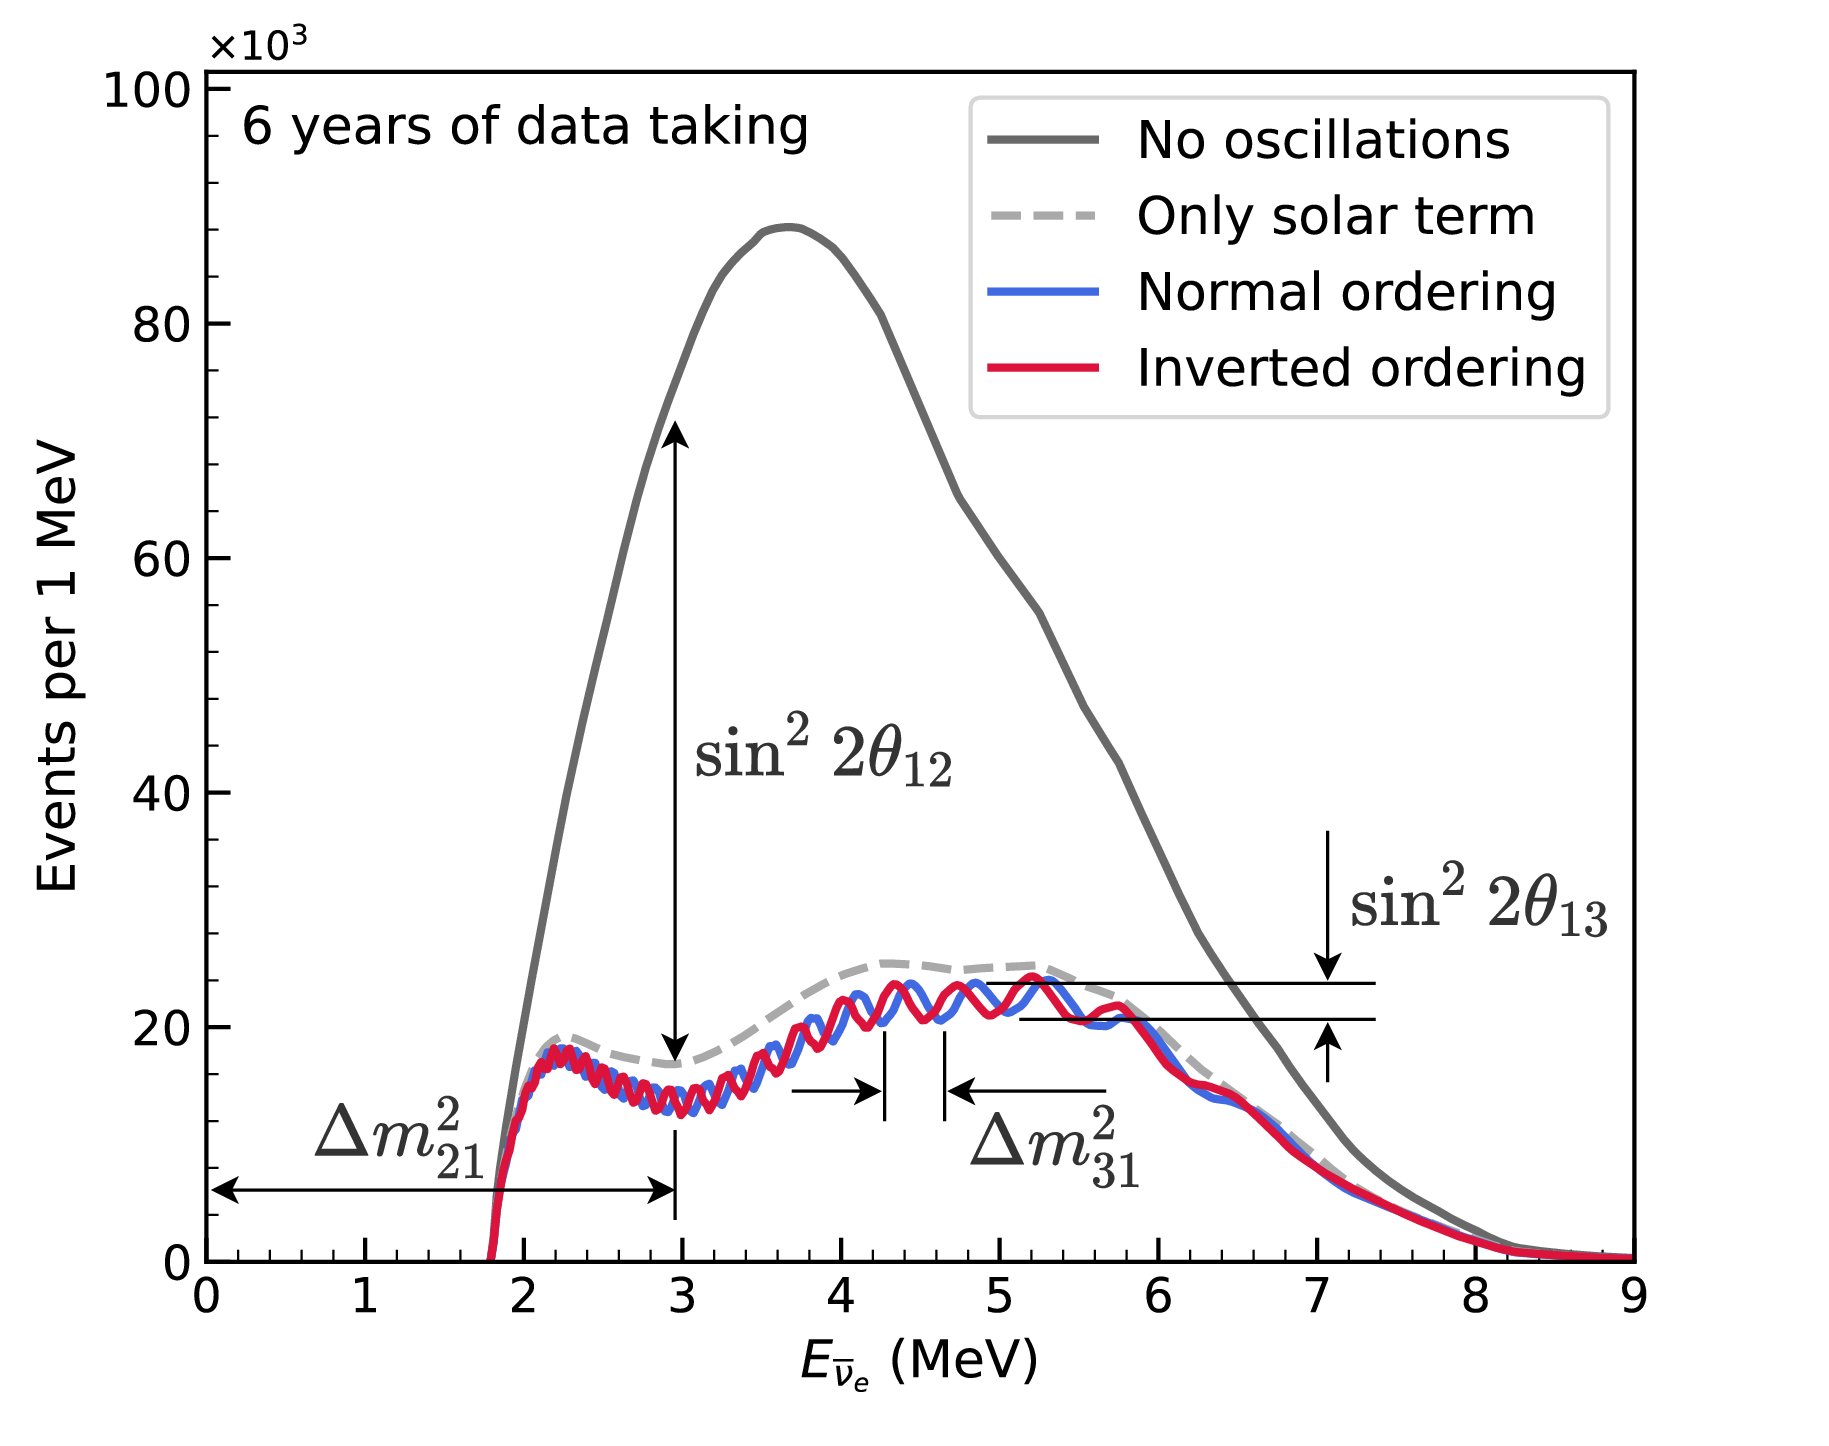
\includegraphics[height=6cm]{images/juno/Spectrum-OscillationsOnly_dm2_31.png}
  \caption{Expected number of neutrinos event per MeV in JUNO after 6 years of data taking. The black curve shows the flux if there was no oscillation. The light gray curve shows the oscillation if only the solar terms are taken in account ($\theta_{12}$, $\Delta m_{21}^2$). The blue and red curve shows the spectrum in the case of, respectively, NO and IO. The dependency of the oscillation to the different parameters are schematized by the double sided arrows. We can see the NMO sensitivity by looking at the fine phase shift between the red and the blue curve.}
  \label{fig:joint_fit:juno-spectrum-oscillation}
\end{figure}
\begin{figure}[ht]
  \centering
  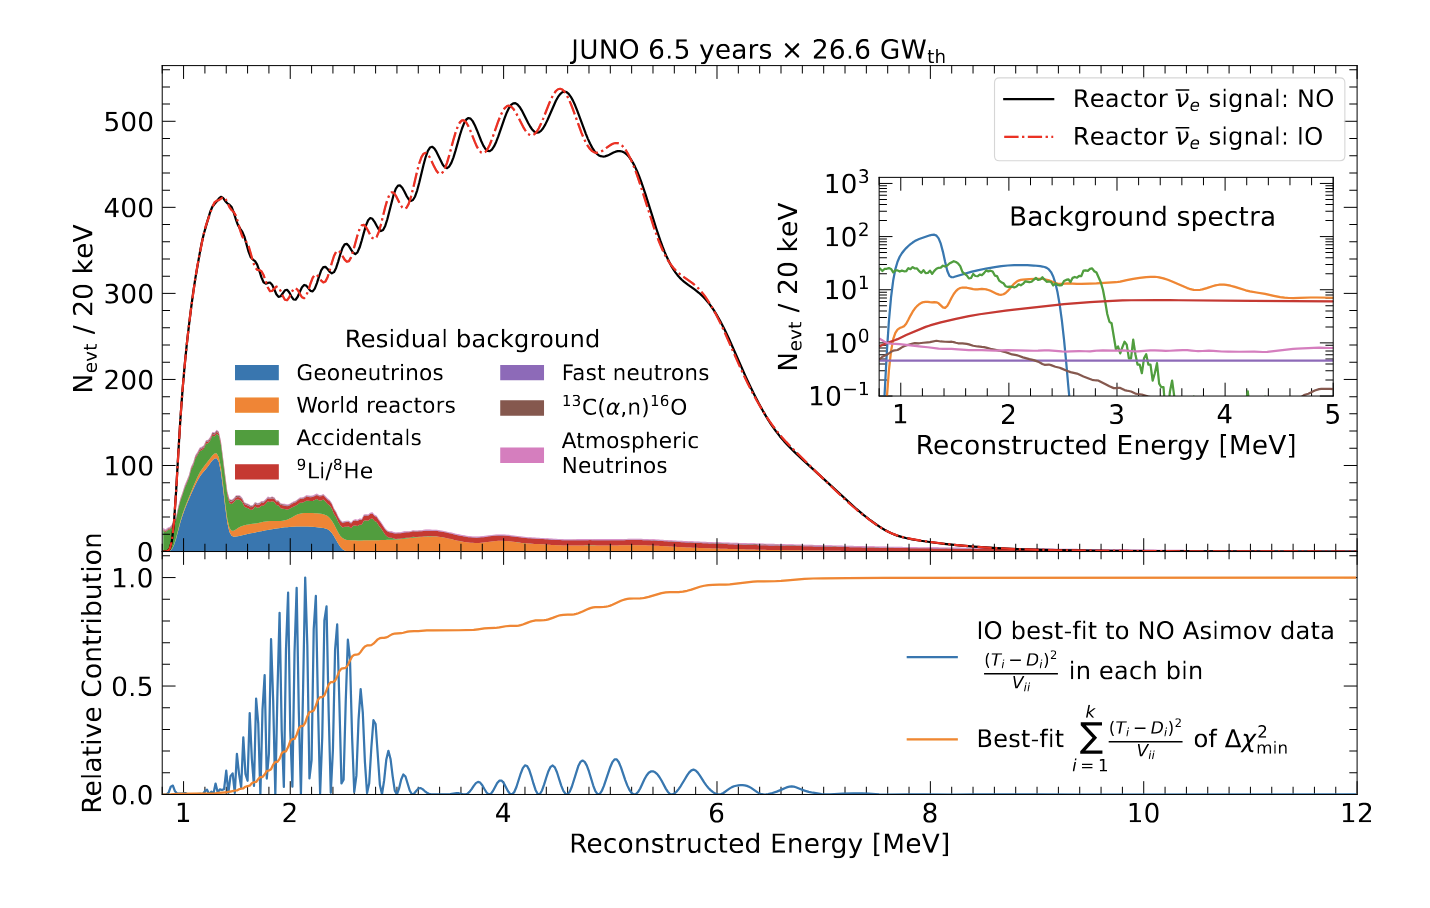
\includegraphics[height=8cm]{images/joint_fit/mass_ordering.png}
  \caption{Oscillated reactor $\bar{\nu}_e$ spectra for the Normal Ordering (Black) and Inverted Ordering (Red) for 6,5 years data taking and a resolution of 3\% without any statistical or systematic fluctuation. Figure from \cite{abusleme_potential_2024}.}
  \label{fig:joint_fit:juno-ordering}
\end{figure}


One of the possible source of non-linearity, which will be used as a reference in this chapter, is the charge non-linearity (QNL) that will be discussed in next section.
Several dual calorimetry techniques can address this issue. Some are calibration techniques, that are also described in section 4.3 of \cite{han_dual_2021} .
More generally, comparing the results of the two systems will allow for the detection of potential issues on the calibration or reconstruction. This is done in this thesis by comparing directly the spectra and oscillation parameters measurements of the two PMT systems. We call this kind of dual calorimetry "Dual calorimetry with neutrino oscillation", since it is based on the visible energy spectra used by the oscillation analysis of reactor antineutrinos.

In this chapter, we explore several ways to perform this comparison. One of them relies on the difference between the values of $\Delta m^2_{21}$, $\sin^2(2\theta_{12})$ measured with the LPMT and the SPMT systems.
Both systems measure them with similar uncertainties. For reasonable values of the QNL, we expect these differences to be smaller than the individual uncertainties. However, the significance of these differences might still be high. Indeed, both systems reconstruct the same events, therefore the same distribution of the true positron energy, as well as the same scintillation photon emission. Therefore,the energy spectra reconstructed by the two systems share a part of their fluctuations. This translates into correlated reconstructed spectra and consequently lead to correlations between the measurements of $\Delta m^2_{21}$ and $\sin^2(2\theta_{12})$. The uncertainty on the SPMT-LPMT difference is largely decreased by this correlation.  Other ways to perform the comparison
(see next sections) all rely the reconstructed spectra, therefore on the evaluation of the correlation between the LPMT and SPMT spectra.

In the next section we will discuss the motivations behind this study. In section \ref{sec:joint_fit:approach},  I present the methods we propose to implement Dual calorimetry with neutrino oscillation, and of the way we estimate their sensitivity. In section \ref{sec:joint_fit:framework}, I present the fit framework used, and then, in section \ref{sec:joint_fit:tech} the technical improvement brought and the difficulties faced during the development. To end this chapter I present the results in \ref{sec:joint_fit:results} and discuss the conclusions and perspectives in \ref{sec:joint_fit:conclusion}.

\section{Motivations}
% II)  Motivations
% --------------------------
%
%   (a) Écart entre les résultats sPMT et LPMT
%       -- Tout écart significatif entre les résultats obtenus avec les deux systèmes signale un problème, et est donc intéressant, quelle que soit l'origine du problème.
%      -- Les deux systèmes ont une sensibilité équivalente à theta_12 et dm2_12. Ce sont donc ces deux paramètres que nous comparerons.
%     -- Pour détecter un écart significatif, on ne peut se contenter de comparer l'écart à la racine de la somme quad des erreurs individuelles. En effet, une grande partie de l'incertitude provient des incertitudes statistiques sur le spectre vrai de l'énergie des antineutrinos. Ce spectre étant le même pour les deux systèmes, les erreurs stats sur spectres reconstruits par les deux systèmes sont très corrélées. Si la reconstruction de l'E avait une résolution et un biais nul dans les deux systèmes, alors l'incertitude statistiques entre les mêmes bins des deux spectres serait 100% corrélée. Dans la réalité, les effets de reconstruction, en partie aléatoires, diminue cette corrélation. Elle reste néanmoins un élément central dans ce travail.
%
%    -- Notre travail dans cette partie de la thèse a été de mettre au point plusieurs tests statistiques pertinents pour détecter un écart entre le système des LPMT et celui des sPMT.
%      + Un premier objectif est de fournir les distributions des tests statistiques dans le cas où il n'existe pas de source de désaccord imprévue entre les deux systèmes. La valeur obtenue dans les données réelles pourra être comparée à ces distributions pour déduire des p-values.
%     + Pour évaluer une sensibilité, nous avons besoin de simuler une différence concrète. Nous choisissons de nous intéresser à un effet plausible, la QNL (voir prochaine sous-section). Nous soulignons cependant que la méthode peut être utile quelle que soit la source d'une différence entre LPMT et sPMT (problème dans la calibration, réglage fin de la simulation insuffisant pour un bon data/MC, etc...)
%
\subsection{Discrepancies between the SPMT and LPMT results}

As discussed in the introduction of this chapter, the SPMT  and LPMT systems will observe the same events. This mean that, after calibration, if the two system show significant differences in their results this is the signal of potential overlook of an effect or problem. Being able to detect such differences is thus crucial, as discussed above, even the smallest deviation from our model could lead to the impossibility to measure the Mass Ordering (MO) or even worse, wrong our measurement.

The two systems are expected to have the same sensitivity to the oscillation parameters $\theta_{12}$ and $\Delta m^2_{21}$ \cite{juno_collaboration_sub-percent_2022}. We will thus rely on the measurement of those two parameters to detect potential discrepancies.

We could just look at the value and compare them to the estimated independent error of the two system, but we believe and will demonstrate in this chapter that the independent study of the two system is missing a lot of informations, and that, by taking into account the statistic and systematic correlations between the two systems, we can produce much more powerful statistical tests.

Our work in this chapter is to develop such tools, which in practice implies to define test statistics. A first step will be to determine the distribution of these test statistics in the case  when no unexpected problem affects the LPMT nor the SPMT problem. This will give us the distribution of those statistical test in absence of discrepancies. Later, the value of the test statistics that we will measure in real data can be compared to these distributions to produce p-values, to judge of the potential present of an unexpected effect.

To evaluate the power of our methods, we need to simulate a concrete difference between the two spectra. We have decided to study a plausible effect, the Charge Non-Linearity (QNL) that is detailed next section.
Note that these tests should in principle be able to detect unexpected effects whatever their source (calibration issues, insufficient simulation tuning, etc.), provided that the distortion caused to the energy spectrum is important enough.

%
%   (b) Explications sur la QNL. (  ~ 1 p)
%
%       -- Rappeler que la réponse en E du détecteur est sujette à plusieurs sources de non linéarité. La principale est la NL dans la scintillation de photons. Une autre source est la QNL.
%
%      -- Définition, origine, etc.
%
%      -- Une façon de modéliser : la formule de Yang sur les Q_LPMT.
%          * Insérer les figures que tu as produites récemment (voir slack le 8 juillet à 17h39 et 17h52) : N_ph/N_ph_qnl vs. Etrue, pour différentes valeurs de gamma_qnl. Cela permet au lecteur de rapidement comprendre l'impact du PB.
%         * Fais le lien entre alpha_qnl et gamma_qnl, pour expliquer que plus tard, on ne testera que avec alpha_qnl, c'est à dire en simulant un effet global sur l'Erec pour générer plus vite.
%         * Dans ces figures, tu t'arrêtes à gamma_qnl = 1% <=> alpha_qnl = 0.3 %, je pense que tu peux aller jusqu'au 5% (regarde ce qui est fait chez Yang et dans la publi multicalo). Aussi bien à 0.5%, qu'à 1% et  qu'à 5%, donne le alpha_QNL correspondant, puis introduis-le dans IBDgen pour produire une spectre oscillé biaisé par la QNL, à comparer dans une figure au spectre sans QNL. Le but est de donner une idée de l'impact sur la NMO.
% En tout cas convaincre qu'il y en a un. Si Steven peut produire un delta-chi2, ce serait super.
%
% Remarques :
%       -- C'est un point important, donc il faut que cela soit auto-contenu au maximum.
%       -- S'inspirer de la publi multicalo, et de la thèse de Yang.
%       -- Citer ces deux sources, mais seulement en complément.
%

\subsection{Charge Non-Linearity (QNL)}
\label{sec:joint_fit:qnl}

The CD energy response is subject to two kinds of non-linearity, the first one is the LS response non-linearity, where the LS photo-production is not linear with the deposited energy as illustrated in figure \ref{fig:juno:nl:gamma}. The LS response is composed of physical non-linearity. Particle interactions in the LS will produce mainly scintillation light, as discussed in section \ref{sec:juno:LS}, but will also produce some Cherenkov light (< 10\% of the collected light). Both mechanisms possess intrinsic non-linearity, for the Cherenkov emission it depends on the velocity of charged particle velocity while the scintillation photon-yield follows a so-called Birk's law with a "quenching" effect depending on the energy and type of particle \cite{particle_data_group_review_2020}. This result in a event-wise non-linearity.


The second type of non-linearity comes from the LPMT charge measurements. When photons hit a PMT and give rise to PEs, a current pulse is formed. In the photon counting regime, simply exceeding a certain threshold allows to conclude that a single photon hit the PMT. When several photons hit the PMT simultaneously, one enters the photon integration regime : the pulse is sampled and integrated over a certain time window to produce a reconstructed charge Q. Calibration methods are applied to determine the relationship between the charge Q and the number of PEs (which is the quantity proportional to the energy deposit one wants to measure). Several effects impact this procedure: the signal pulse can fluctuate and be distorted between two events where the same number PEs occured; the PMT gain might not be linear as a function of the number of photons that hit the PMT; the charge reconstruction algorithm is not supposed to be perfect, and its results are further affected by electronic noise and inter-channel cross-talk. The impact of these effects grows with the number of PEs.

Precedent studies \cite{han_dual_2021} suggest a model for the channel-wise QNL:
\begin{equation}
  \label{eq:joint_fit:gamma_yang}
  \frac{Q_{rec}}{Q_{true}} = \frac{-\gamma_{qnl}}{9} Q_{true} + \frac{\gamma_{qnl} + 9}{9}
\end{equation}
where $Q_{rec}$ is the reconstructed number of PE by the PMT, $Q_{true}$ is true number of PE that hit the PMT, and $\gamma_{qnl}$ is a factor representing the amplitude of the non-linearity.

Studies at previous experiments, like Daya Bay, concluded that the best reachable control of QNL in the 1-10 PEs range was $\gamma_{qnl}=0.01$ \cite{collaboration_high_2019}.
As already mentionned in section \ref{sec:juno:LPMT}, JUNO LPMTs operate in a larger range : 1-100 PEs (See also table \ref{tab:joint_fit:charge_frac}). In such a case, a realistic value of $\gamma_{qnl}$ is not known.

\begin{table}[ht]
  \centering
  \begin{tabular}{c|c|c|c|c|c|c|c}
        &1PE &2$\sim$5PE& 5$\sim$10PE & 10$\sim$20PE & 20$\sim$50PE & 50$\sim$100PE & >100PE \\
      \hline
    LPMT &42.56\% & 40.54\% & 8.74\% & 5.12\% & 2.80\% & 0.24\% & 0.003\% \\
    SPMT &95.19\% & 4.80\%  & 0.01\% & 0\%    & 0\%    & 0\%    & 0\% \\
    \hline
  \end{tabular}
  \caption{The charge fraction in terms of the number of PE collected at the single PMT for the reactor $\bar{\nu}_e$ IBD events. Table taken from \cite{han_dual_2021}}
  \label{tab:joint_fit:charge_frac}
\end{table}

The event-wise impact resulting from the channel-wise QNL can be parameterised this way :
\begin{equation}
  \label{eq:joint_fit:alpha_yang}
  \frac{E^{rec}_{vis}}{E^{true}_{vis}} = \frac{-\alpha_{qnl}}{9} E^{true}_{vis} + \frac{\alpha_{qnl} + 9}{9}
\end{equation}
In JUNO, the visible energy is proportional to the number of emitted photons per unit energy deposit. It includes the physical non linearities.
In the equation above $E_{vis}^{true}$ is this visible energy, while $E_{vis}^{rec}$ is what it becomes when the reconstructed charges found in an event are modified according to Eq. \ref{eq:joint_fit:gamma_yang}.

\begin{figure}[ht]
  \centering
  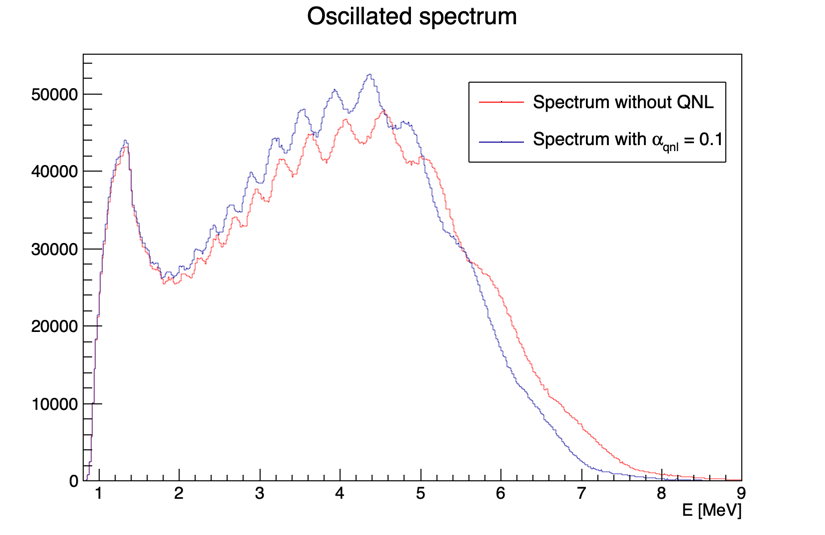
\includegraphics[height=5cm]{images/joint_fit/spectrums.png}
  \caption{Two oscillated spectra of 1e7 event expected in JUNO. In red the spectrum without supplementary QNL. In blue the same spectrum but where an event-wise QNL $\alpha_{qnl} = 10\%$ is introduced.}
  \label{fig:joint_fit:spectrums_comp}
\end{figure}


An example is shown on Fig. \ref{fig:juno:instr_nl}, where we show the $E^{rec}_{vis}/E_{true}^{vis}$ ratio for several samples of uniformly distributed electron events, generated with various values of $E_{vis}^{true}$.
Here, an extreme value $\gamma_{qnl}=0.05$ was assumed. On can see on Fig. \ref{fig:juno:instr_nl} that it corresponds to a 2\% effect at 8 MeV, equivalent to $\alpha_{qnl} = 0.025$.

This example is from  from references \cite{han_dual_2021}, which aimed at demonstrating the potential of the dual calorimetry calibration method mentioned in section
\ref{sec:juno:instr_nl}. If it works as hoped, the residual event-wise QNL effect will be below 0.3\%. In this chapter, we propose methods todetect residuals higher than this.

Fig. \ref{fig:joint_fit:gamma_v_alpha} show several other examples with varying $\gamma_{qnl}$ values, and
the corresponding values of $\alpha_{qnl}$.
Using 1M events from the JUNO official simulation J23.0.1-rc8.dc1 (released on 7th January 2024), we
simulated events up to the photon collection in LPMTs and introduced an additional channel-wise
QNL by using the equation 7.1 to modify the number of collected photons.

\begin{figure}
  \centering
  \begin{subfigure}[t]{0.48\linewidth}
    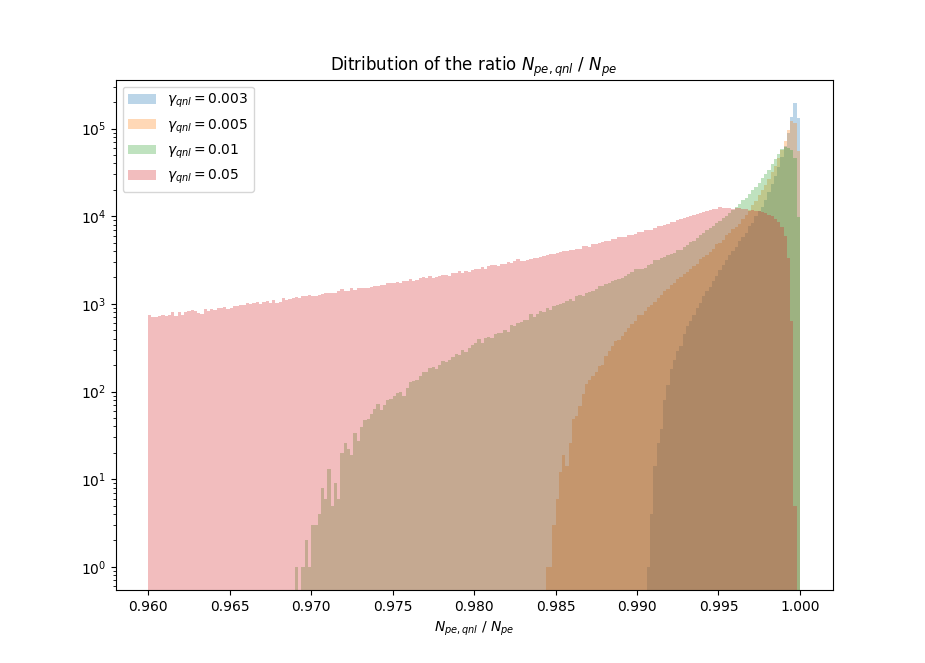
\includegraphics[width=\linewidth]{images/joint_fit/gamma_eff.png}
    \caption{Distribution of ratio of collected nPE after the additional QNL over the number of nPE that would be collected for different $\gamma_{qnl}$. We select event with an interaction radius $R < 4$m to not be affected by the non-uniformity.}
    \label{fig:joint_fit:ratio_distrib}
  \end{subfigure}
  \hfill
  \begin{subfigure}[t]{0.48\linewidth}
    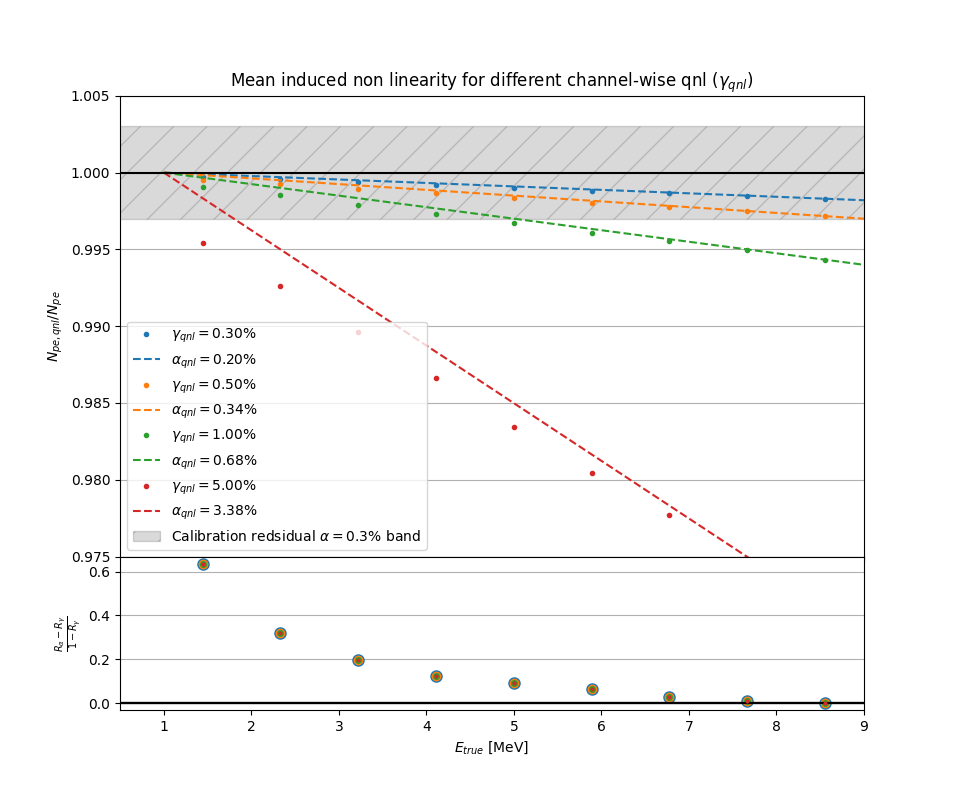
\includegraphics[width=\linewidth]{images/joint_fit/gamma_to_alpha.png}
    \caption{Ratio of collected nPE after the additional QNL over the number of nPE that would be collected at different energies. We select event with an interaction radius $R < 4$m to not be affected by the non-uniformity. The dots represent the mean of the distributions in figure \ref{fig:joint_fit:ratio_distrib} and the dashed line are the equivalent event-wise non-linearity from eq \ref{eq:joint_fit:alpha_yang}. The hatched zone is the residual non-linearity expected after calibration \cite{juno_collaboration_calibration_2021}.}
    \label{fig:joint_fit:gamma_v_alpha}
  \end{subfigure}
  \caption{}
\end{figure}

In figure \ref{fig:joint_fit:ratio_distrib} we show the distribution of the ratio $\frac{Q_{rec}}{Q_{true}}$ for central events ($R < 4$m) and different values of $\gamma_{qnl}$. In figure \ref{fig:joint_fit:ratio_distrib}, we show the mean of this distribution as a function of the energy. We also present the effective $\alpha_{qnl}$ for each value of $\gamma_{qnl}$. We observe that using the event-wise QNL is equivalent to the mean behavior of using channel-wise QNL.

When using channel-wise non-linearity, we need to simulate a number of PE per LPMT, the process can be quite tedious if we want a realistic simulation. So in this study we are only using event-wise non-linearity to make the process simpler. This event-wise non-linearity will be characterized by $\alpha_{qnl}$ in this work.

%  (c) Blinding ?
%  L: Pas expert du sujet (mais alors pas du tout). Je me souviens de la discussion avec steven ou on pourrait ainsi appliquer nos outils avant l'unblidding et ainsi verifier que tout vas bien avant de regarder les resultats ?
%
%
%  (d) Motivations techniques
%
%       -- À compléter à partir de mes notes.
%          Tourne autour de la capacité, utile en général, à réaliser un fit joint.
%  L: En gros dire que c'est pratique de savoir le faire ?

\section{Approach}
\label{sec:joint_fit:approach}

In this section, we detail the testing procedure for each of our tools.

% III) Démarche
% -----------------------
%
%   (a) Simulation d'échantillons toys.
%
%          --- C'est la base de cette étude.
%          --- Dans chaque toy, nous générons un spectre vrai de l'E_nu qui est le point de départ commun de la production des deux spectres reconstruits des LPMT et des sPMt.
%          --- Puis nous ajoutons de façon simplifiée (pas nécessaire d'en dire plus ici, voir la sous - section sur IBDgen) les effets de reco pour avoir dans chaque toy deux spectres.
%          --- Nous étudions plus loin l'effet de la l'exposition sur la sensibilité de la méthode. Donc cet exercice est répété pour plusieurs statistiques (100 jours, 1 an, 2 ans, 6 ans).

\subsection{Data production}

\subsubsection{IBD spectra}

The first step involves generating the data on which we our tools will be tested. In this study we use Monte-Carlo toys. For each toy we generate a $\bar{\nu}_e$ energy spectrum from the Taishan, Yangjiang and Dayabay nuclear power plants, the reactors used as source for the NMO analysis. The reactors parameters comes from JUNO official database, which shared among all physics analysis, the JUNO common inputs. This provides the initial spectra for the LPMT and SPMT systems. We then incorporate physic effects such as the LS non-linearity etc... (more details in section \ref{sec:joint_fit:framework:ibd-gen}). Finally, we apply the reconstruction resolution for each system to their respective spectra, resulting in the final LPMT and SPMT spectra.

We will study the effect of exposure on our methods at different threshold: 100 days, 1 year, 2 year and finally 6 years which is the nominal data taking period for the NMO analysis.

These spectra are generated for different QNL, $\alpha_{qnl} = 0$ (no spectrum distortion) and for $\alpha_{qnl} \in \{0.01, 0.005, 0.003, 0.002, 0.001\}$. As a reminder, the calibration guarantees a residual event-wise non-linearity of $\alpha_{qnl} \leq 0.003$ \cite{juno_collaboration_calibration_2021}.

The first test does not require any fitting, we are just comparing the LPMT and SPMT spectra using the expected statistical correlation matrix in the case $\alpha_{qnl} = 0$. For details about the generation of this correlation matrix, refer to section \ref{sec:joint_fit:cov_mat}. This test is the spectrum $\chi^2$ or $\chi^2_{spe}$. In this test we compute a $\chi^2$ representing the compatibility between the LPMT and SPMT spectra:
\begin{align}
  \Delta_i &= h_{L,i} - h_{S,i} \\
  U &= A V A^T \\
  \chi^2_{spe} &= \vec{\Delta}^T U^{-1} \vec{\Delta}
\end{align}
Where $h_{L,i}$ and $h_{S,i}$ are the contents of the $i$th bin of the LPMT and SPMT spectra respectively. $V$ is the covariance matrix of the LPMT + SPMT spectra. $A$ is a transformation matrix defined as:
\begin{equation}
  A_{ij} = \frac{\partial \Delta_i}{\partial h_j} = \frac{\partial(h_{L, i} - h_{S, i})}{\partial h_j}
\end{equation}
Thus, $A_{ij} = 1$ if $i = j$, and $A_{ij} = -1$ if $j$ is the SPMT bin corresponding to the $i$ LPMT bin.

This $\chi^2_{spe}$ is minimal when the statistic between the bins of the LPMT and SPMT spectra follow the covariance matrix $V$. By looking at the distribution of this $\chi^2_{spe}$ when $\alpha_{qnl} = 0$ we can produce p-values for the values found when $\alpha_{qnl} \neq 0$.

\subsubsection{Background spectra}

The JUNO common inputs provide only LPMT background spectra. These background spectra are already smeared by the LPMT resolution and thus need to be regenerated to be smeared to account for the SPMT resolution. Fortunately the SPMT resolution is greater than that of the LPMT, allowing us to apply additional smearing to the spectrum using
\begin{equation}
  \label{eq:joint_fit:oversmear}
  S(E) = L(E) \star \frac{1}{\sqrt{|\Delta \sigma^2|} \sqrt{2\pi}} e^{-\frac{E^2}{2|\Delta \sigma^2|}}; ~ |\Delta \sigma^2| = \sigma_L^2 - \sigma_S^2
\end{equation}
Where $S(E)$ is the SPMT spectrum, $L(E)$ the LPMT spectrum, $\sigma_L$ and $\sigma_S$ the LPMT and SPMT resolution respectively. This formula is valid under the assumption that the LPMT and SPMT smearing are gaussian and that the LPMT and SPMT have the same bias. Those two assumptions are valid in the context of the IBD spectrum production as detailed in section \ref{sec:joint_fit:framework:ibd-gen}.
The demonstration of equation \ref{eq:joint_fit:oversmear} can be found in annex \ref{sec:annex:oversmearing}.


%   (b) Fits séparés
%     --- Fit individuel LPMT puis sPMT dans chaque toy.
%     --- Les N_toys résultats permettent d'établir la corrélation entre les param d'oscillations mesurés par les deux fits quand la génération ne suppose pas d'effets de reco imprévus.
%          => Description du test statistiques

\subsection{Individual fits}

Each of the spectra, LPMT and SPMT, are then fitted individually with and without the presence of QNL over multiples toys. The results allow us to compute the correlation between the oscillations parameters measured by both of the systems when there is no QNL allowing us to compute a $\chi^2$ representing the compatibility between the measurements of the systems. Because the SPMT system is not sensible to the oscillation parameters $\Delta m^2_{31}$ and $\theta_{13}$, the test is only done on the oscillation parameters $\theta_{12}$ and $\Delta m^2_{21}$. We can thus produce the individual chi square $\chi^2_{ind}$
\begin{align}
  \Delta_\lambda &= \lambda_{L} - \lambda_{S} \\
  \vec{\Delta} &= [ \Delta_{\theta_{12}} ~ \Delta_{\Delta m^2_{21}} ] \\
  U &= A V A^T \\
  \chi^2_{ind} &= \vec{\Delta}^T U^{-1} \vec{\Delta}
\end{align}
where $\lambda_{L}$ and $\lambda_{S}$ are the measured parameters by the LPMT and SPMT systems respectively. The different $\lambda$ considered are $\theta_{12}$ and $\Delta m^2_{21}$. $V$ here is the $4\times 4$ covariance matrix between the parameters $\theta_{12, L}$, $\Delta m^2_{21, L}$, $\theta_{12, S}$ and  $\Delta m^2_{21, S}$. $A$ is the transformation matrix that allow us to compute the covariance matrix de $\vec{\Delta}$ from $V$ following
\begin{equation}
  A_{ij} = \frac{\partial \Delta_i}{\partial j}; ~ i \in \{ \theta_{12}, \Delta m^2_{21} \}; ~ j \in \{ \theta_{12, L}, \Delta m^2_{21, L}, \theta_{12, S}, \Delta m^2_{21, S} \}
\end{equation}

Same as described above, by comparing the distribution of this $\chi^2_{ind}$ when $\alpha_{qnl} = 0$ and $\alpha_{qnl} \neq 0$ we can compute the power of this test in term of p-values.

%
%  (c) Fit joint
%
%     --- Un fit de chi2, ajustant aux deux spectres 2 pdf distinctes (par la modèle de reconstruction qu'elles supposent).
%
%     --- Les paramètres ajustés par le fit sont :  ...
%
%     --- Les paramètres fixes, ou contraints par un pull term : ...
%
%     --- Les pdf sont distinctes, mais les valeurs des paramètres d'oscillations sont communes aux deux fits.
%
%     --- Pour tenir compte d'un biais dû à un effet de reco imprévu, delta_th et delta_dm ajoutés à th12 et dm2_12 dans la pdf appliquée au spectre LPMT.
%
%     --- Nous avons là par défaut deux spectres de 410 bins, donc un spectre global de 820 bins. Nous effectuons un fit de chi2 : besoin d'une matrice de corrélation. Dans la plupart des fits joints entre spectres (comme lorsque l'on combine plusieurs expériences) la matrice de covariance statistique totale (celle entre les 820 bins dans notre cas) est diagonale car les différents spectres sont indépendants statistiquement. Là, nous avons pour défi de déterminer les corrélations statistiques entre les deux spectres. Expliqué en section xx.
%
%
%    => La statistique de test.

\subsection{Joint fit}

\subsubsection{Standard joint fit}

The final step is to produce a joint fit between the two spectra. In this case we adjust our model, the oscillated spectrum, over two spectra as the same time. We minimize a $\chi^2_{joint}$ defined over the two spectra, the LPMT and SPMT one
\begin{align}
  \label{eq:joint_fit:pearson}
  \Delta_i &= D_{i} - T_{i} \\
  \chi^2_{joint} &= \vec{\Delta}^T V^{-1} \vec{\Delta}
\end{align}
where $D_{i}$ is the content of the $i$th bin measured, from the data, and $T_{i}$ is the theoretical number of event in this bin. $V$ is the covariance matrix of our spectrum.

$T$ is the fitted function and depend on multiple parameters
\begin{itemize}
  \item The oscillation parameters $\theta_{12}$, $\Delta m^2_{21}$, $\theta_{13}$ and $\Delta m^2_{31}$. Those parameters can be free, have a pull term or be fixed during the fit.
  \item We take into account in the data production the matter effect and parametrize it by the parameter $\rho$, the effective rock density between the reactors and the experiment. Same as the oscillation parameters, this parameter can be free, pulled or fixed.
  \item The exposure of the considered data which is just a normalization factor in front of the theoretical spectrum. This parameter is fixed at the start of the fit.
\end{itemize}

In the standard joint fit, the free parameters are $\sin^2(2\theta_{12})$, $\Delta m^2_{21}$ and $\Delta m^2_{31}$. $\sin^2(2\theta_{13})$ is fixed to the PDG nominal value. For simplicity, we refer to $\sin^2(2\theta_{12})$ and $\sin^2(2\theta_{13})$ as $\theta_{12}$ and $\theta_{13}$ respectively.

Both of the LPMT and SPMT systems are sensitive to $\theta_{12}$ and $\Delta m^2_{21}$, thus these parameters are totally free and start at the PDG nominal value. Only the LPMT system is sensitive to $\Delta m^2_{31}$, we let it free so we can observe the effect of the deformation on it while the solar parameters $\theta_{12}$, $\Delta m^2_{21}$ are constrained by the SPMT system. To prevent $\Delta m^2_{31}$ to take absurd value, we add a pull term using the PDG nominal value and errors. The PDG nominal values used in this study can be found in table \ref{tab:joint_fit:pdg_value}.
\begin{equation}
  \chi^2_{joint} = \vec{\Delta}^T V^{-1} \vec{\Delta} + \frac{\Delta m^2_{31} - \Delta m^2_{31,PDG}}{\sigma_{31, PDG}}
\end{equation}


\begin{table}
  \centering
  \begin{tabular}{c|c|c|c}
    $\sin^2(2\theta_{12})$    & $\Delta m^2_{21}$                       & $\Delta m^2_{31}$      & $\sin^2(2\theta_{13})$ \\
    \hline
    $0.851^{+0.020}_{-0.018}$ & $7.53 \pm 0.18 \times 10^{-5}$ eV$^2$   & $2.5283 \pm 0.034 \times 10^{-3}$ eV$^2$  & $0.0.8523 \pm 0.00268$
  \end{tabular}
  \caption{Nominal PDG2020 value \cite{particle_data_group_review_2020}. All value are reported assuming Normal Ordering.}
  \label{tab:joint_fit:pdg_value}
\end{table}



$\theta_{13}$ is the parameter on which we are least accurate. It's fixed to nominal value to prevent degeneracy (table \ref{tab:joint_fit:pdg_value}).

The covariance matrix is produced from a correlation matrix $C$
\begin{equation}
  V_{ij} = \sigma_{i} \sigma_{j} C_{ij}
\end{equation}
where $\sigma_{i}$ is the uncertainty on the number of event in the $i$th bin. We consider in this study that the content of each bin follow a Poisson statistic, thus the uncertainty is $\sigma_i = \sqrt{N_i}$ where $N_i$ is the content of the $i$th bin. The bin content used for the uncertainty can come from two sources: the data and the theoretical spectra $\sigma_i = \sqrt{D_i}$ (Pearson test) and $\sigma_i = \sqrt{T_i}$ (Neyman test). Precedent studies have show that both Pearson and Neyman tests show bias at low statistic, we thus use the Pearson V test where
\begin{equation}
  \label{eq:joint_fit:pearsonV}
  \chi^2_{joint} = \vec{\Delta}^T V^{-1} \vec{\Delta} + \frac{\Delta m^2_{31} - \Delta m^2_{31,PDG}}{\sigma_{31, PDG}} + \mathrm{ln} | V |
\end{equation}
and the covariance matrix $V$ is computed using the data spectrum for the uncertainty.

The estimation of the covariance is crucial in this study as the strength of this test rely on the systematic and statistical correlations between the LPMT and SPMT spectrum. The generation methods and results of this matrix is detailed in section \ref{sec:joint_fit:cov_mat}.

\subsubsection{Delta joint fit}

Using the same structure we define a second joint fit, the Delta joint fit where, in addition to everything that was discussed above, we add two other parameters $\delta \theta_{12}$ and $\delta \Delta m^2_{21}$ and split the theoretical $T(\theta_{12}, \Delta m^2_{21}, ...)$ spectrum in two
\begin{equation}
\begin{split}
           &T_{LPMT} \equiv T(\theta_{12} + \delta \theta_{12}, \Delta m^2_{21} + \delta \Delta m^2_{21}, ...) \\
           &T_{SPMT} \equiv T(\theta_{12}                     , \Delta m^2_{21}                         , ...)
\end{split}
\end{equation}

If the there is no additional distortion between the LPMT and the SPMT spectra, the fit should converge to $\delta \theta_{12} = \delta \Delta m^2_{21} = 0$. By observing the dispersion of those parameters we can define the probability $P(\alpha_{qnl} = 0 | (\delta \theta_{12}, \delta \Delta m^2_{21}))$ and use the median value of $(\delta \theta_{12}, \delta \Delta m^2_{21})$ when $\alpha_{qnl} \neq 0$ to define a p-value.

The last test we explore in this thesis is to fit the same spectrum with the Standard Joint fit, that we consider as the hypothesis without distortion $H_0$, and the Delta Joint fit, designated as the $H_1$ hypothesis. By looking at the dispersion of $\chi^2_{joint,H_0} - \chi^2_{joint,H_1}$ we can extract a sensitivity to potential distortion.

\subsection{Data and theoretical spectrum generation}
\label{sec:joint_fit:data_gen}

To implement the joint fit, we have technically two data spectra and two theoretical spectra. The data in this study are produced using an IBD generator \textit{IBD gen}, see section \ref{sec:joint_fit:framework:ibd-gen}. The theoretical spectrum are produced the same way as data spectrum but with much higher statistics, $10^7$ events to compare with the $\approx 10^5$ events for 6 years statistic. The two spectrum, that we get as a collection of events, are binned in two histograms from 0.8 to 9 MeV of reconstructed energy with bins of 0.02 MeV each, resulting in 410 bins per spectrum. An illustration of the theoretical spectrum can be found in figure \ref{fig:joint_fit:delta:theo}. The low number of events in the tail of the spectrum can cause instability due to the low statistic, we thus cut the spectrum at 7.5 MeV / 335 bins for the fit.

\begin{figure}
  \centering
  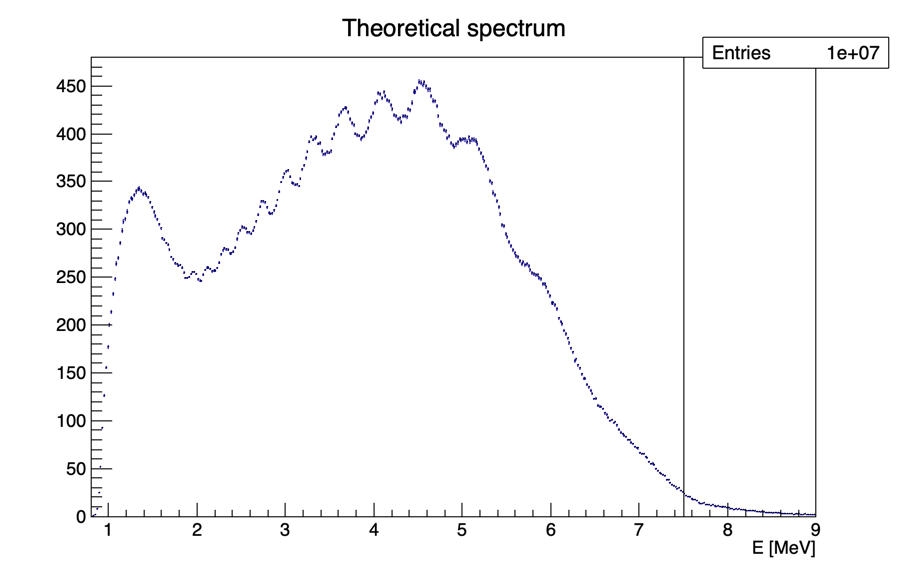
\includegraphics[height=6cm]{images/joint_fit/theoretical_spectrum.png}
  \caption{Theoretical LPMT spectrum at nominal oscillation values binned using 410 bins from 0.8 to 9 MeV. It is rescaled to 6 years statistic. The black line represent the 335 bin cut}
  \label{fig:joint_fit:delta:theo}
\end{figure}

All the IBD spectra presented and used in this study are produced assuming Normal Ordering using the PDG nominal value \cite{particle_data_group_review_2020} for the oscillation parameters. Those values are reported in table \ref{tab:joint_fit:pdg_value}.

%
%   (d) Les suppositions
%
%       --- Nous travaillons en traitant que des erreurs statistiques. Cela se justifie pour un travail exploratoire dans la mesure où une grande partie des effets syst sont totalement corrélés (ceux qui affectent le spectre vrai des neutrinos et des bruits de fond, voir table XX -- systèmatiques du papier Subpercent. )
%
%        --- L'essentiel de nos résultats supposent les effets de détection décorrélés entre LPMT et sPMT. Ils sont par ailleurs introduits de manière simpliste (simple tirage gaussien supposant une résolution gaussienne ne dépendant pas de la position de l'intéraction dans le détecteur --conforme à la publi Subpercent et à la dernière publi NMO). Ce choix se justifie pour un travail exploratoire par la nécessité de produire un grand nombre de toys malgré une puissance de calcul limitée. Un premier raffinement de cette approche tenant compte des corrélations entre les deux reconstructions est présenté en fin de chapitre. Il s'appuie sur la simulation complète du détecteur, et sur notre algo CNN de reco sPMT, le seul disponible à ce jour.
%
%        ---- La QNL est introduite de manière un peu simpliste pour l'instant (appliquée à nouveau juste en fonction de l'énergie de l'IBD). Rappeler que tu as tout de même établi une correspondance (alpha_qnl vs. gamma_qnl) en commençant à faire le boulot qu'il faudrait faire : l'appliquer au niveau des PMT (ce qui tient compte des effets de position de l'intéraction).

\subsection{Limitations}

In this work we are only working considering the statistical errors. We can ignore systematic effects, such as effects that would affect the neutrino spectrum or the background spectrum, as they are entirely correlated between the two systems. The details of those systematic effects can be found in \cite{juno_collaboration_sub-percent_2022}.

Most of our results assume decorrelated detection effects between the SPMT and LPMT systems. Their respective reconstruction effects are simulated using simple gaussian drawing on the resolution, independently from the event position. This approach was used in previous sensitivity and precision studies \cite{juno_collaboration_sub-percent_2022, abusleme_potential_2024}. The potential effect of those reconstruction effects and a first attempt to take them into account are explored in section \ref{sec:joint_fit:cov_mat}.

Even if the goal of this work is to propose deformation agnostic tools, the QNL we use in this study is simplistic as we consider event-wise, position uniform deformation. We show in figure \ref{fig:joint_fit:ratio_distrib} and \ref{fig:joint_fit:gamma_v_alpha} that event-wise QNl is equivalent to the mean behaviour of channel-wise QNL but a more complete study would simulate channel-wise deformation for each event.

\section{Fit software}
\label{sec:joint_fit:framework}

In this section, I describe the ft framework that was used in this study. The software is composed of two parts as illustrated in figure \ref{fig:joint_fit:framework}: A standalone part composed of ROOT \cite{brun_root-projectroot_2022} macros, and the Avenue framework.

The Avenue framework is responsible for the spectrum and configuration reading, transforming the raw collection of events into spectra, managing the physics effect such as the oscillation and computing and minimizing the $\chi^2$ with the help of the RooFit library. The macros are invoking, if necessary, the Avenue framework and are the entry point for fitting, generating the necessary inputs quantity such as the spectra and correlation matrix, analysing the fit results and managing jobs for distributed computing.

\begin{figure}[ht]
  \centering
  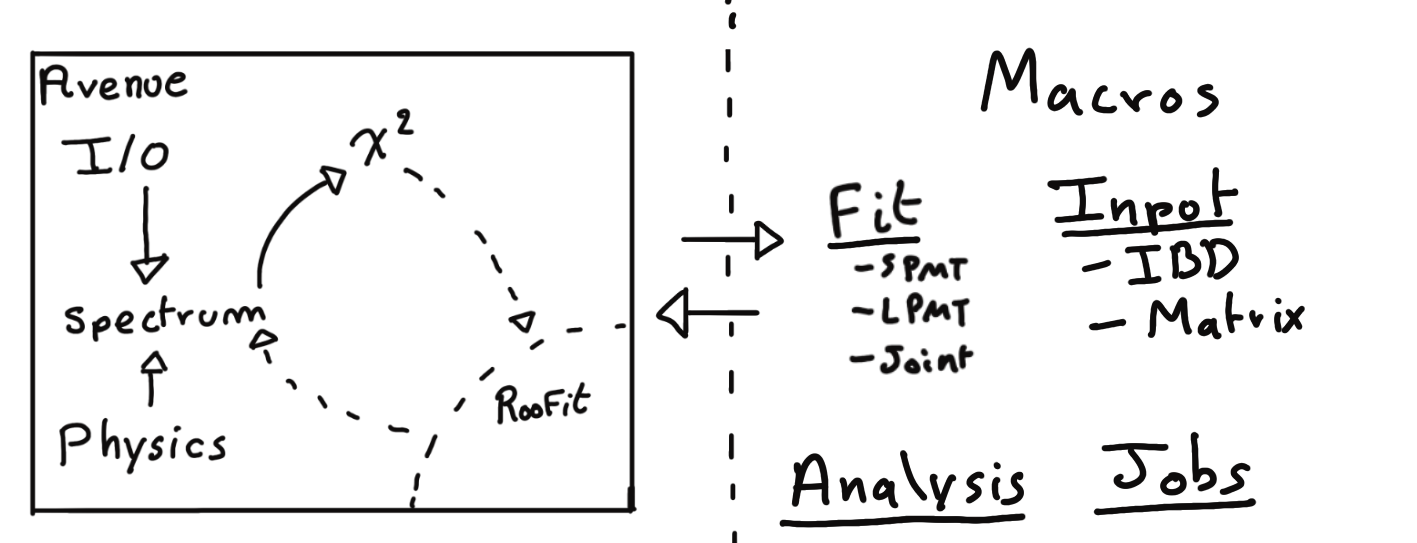
\includegraphics[height=6cm]{images/joint_fit/fit_framework.png}
  \caption{Schematic description of the fit framework}
  \label{fig:joint_fit:framework}
\end{figure}

In this section we will focus on the IBD generator in section \ref{sec:joint_fit:framework:ibd-gen} and the fit macro in itself in section \ref{sec:joint_fit:framework:fit}.
% IV) Le framework de fit.
% ---------------------------------------
%
% ... Description plus ou moins détaillée suivant qu'il a, ou non, déjà été décrit ailleurs...
%
%   (a) Introduction avec rapide overview
%
%
%   (b) La partie standalone : IBD-gen
\subsection{IBD generator}
\label{sec:joint_fit:framework:ibd-gen}

The IBD generator is a standalone generator used to produce oscillated and non oscillated spectra as the one seen by the JUNO experiment. It takes as inputs physics parameters and a collection of histograms, values and function provided by JUNO to its analysis groups, referred as the JUNO common inputs.

Options allow to enable or disable effects such as non-uniformity and non-linearity. It finally take as an argument the number of events to generate $N_{evt}$. Optionally, we generate an effective number of events $N$ by drawing in a Poisson distribution of mean $N_{evt}$.

Then for each event we
\begin{enumerate}
  \item Choose randomly, following the reactor power fraction, the source reactor of the neutrino.
  \item Generate a random interaction position in the detector following a uniform distribution over the detector volume.
  \item Draw a random neutrino energy $E_{\nu}$ from the expected neutrino emission spectrum of every reactor. This spectrum is computed by:
    \begin{enumerate}
      \item Computing the power spectrum of each isotopes $^{235}$U, $^{238}$U, $^{239}$Pu, $^{241}$Pu using the Huber-Mueller model \cite{huber_determination_2011, mueller_improved_2011}.
      \item Summing the contribution of each isotopes following the respective fission fraction [0.58, 0.07, 0.30, 0.05] as reported in \cite{ma_improved_2013}.
      \item The power of each reactor is then adjusted by their distances from the detector, the detector efficiency and their mean duty cycle (11 of 12 month).
      \item The total spectrum is then finally adjusted by taking into account the correction of the Day Bay bump \cite{daya_bay_collaboration_measurement_2016}, adjustment due to spent nuclear fuel and due to the non-equilibrium.
    \end{enumerate}
  \item \textit{(Optional)} Compute the survival probability due to oscillation at nominal oscillation parameters value. If the neutrino does not survive, the event is rejected and the algorithm restart from step (1).
  \item Compute the emitted positron energy $E_{pos}$ from the mass difference. If the neutrino does not have enough energy reject the event and start from step (1).
  \item Compute the deposited energy $E_{dep}$ by incrementing $E_{pos}$ by 511 keV to account for the positron annihilation. We do not consider cases where some of the energy leak outside of the detector (positron or annihilation gammas escaping the CD).
  \item Correct the deposited energy with the expected event-wise non-linearity from \cite{juno_collaboration_calibration_2021} to obtain the visible energy $E_{vis}$.
  \item \textit{(Optional)} Add a custom non-linearity as described in section \ref{sec:joint_fit:qnl}. This non linearity is characterized by $\alpha_{qnl}$ to obtain $E_{\alpha}$.
  \item Finally, using the expected resolution of the LPMT and SPMT systems,  provided in the JUNO common inputs, we draw from a gaussian characterized by those resolution the reconstructed energy $E_{rec}$ or $E_{lpmt}$ and $E_{spmt}$ for each systems. The resolutions are provided as ABC parameters using
    \begin{equation}
      \frac{\sigma E_{vis}}{E_{vis}} = \sqrt{\bigg(\frac{A}{\sqrt{E_{vis}}}\bigg)^2 + B^2 + \bigg(\frac{C}{E_{vis}}\bigg)^2}
    \end{equation}
    where A is the term driven by the Poisson statistics of the total number of detected photoelectrons, C is dominated by the PMT dark noise, and B is dominated by the detector’s spatial non-uniformity. The relative and absolute resolutions of the LPMT and SPMT systems are illustrated in figure \ref{fig:joint_fit:system_resolution}.
\end{enumerate}

The events are stored as n-tuples and are not yet binned at the end of the generator.

\begin{figure}[ht]
  \centering
  \begin{subfigure}[t]{0.48\linewidth}
    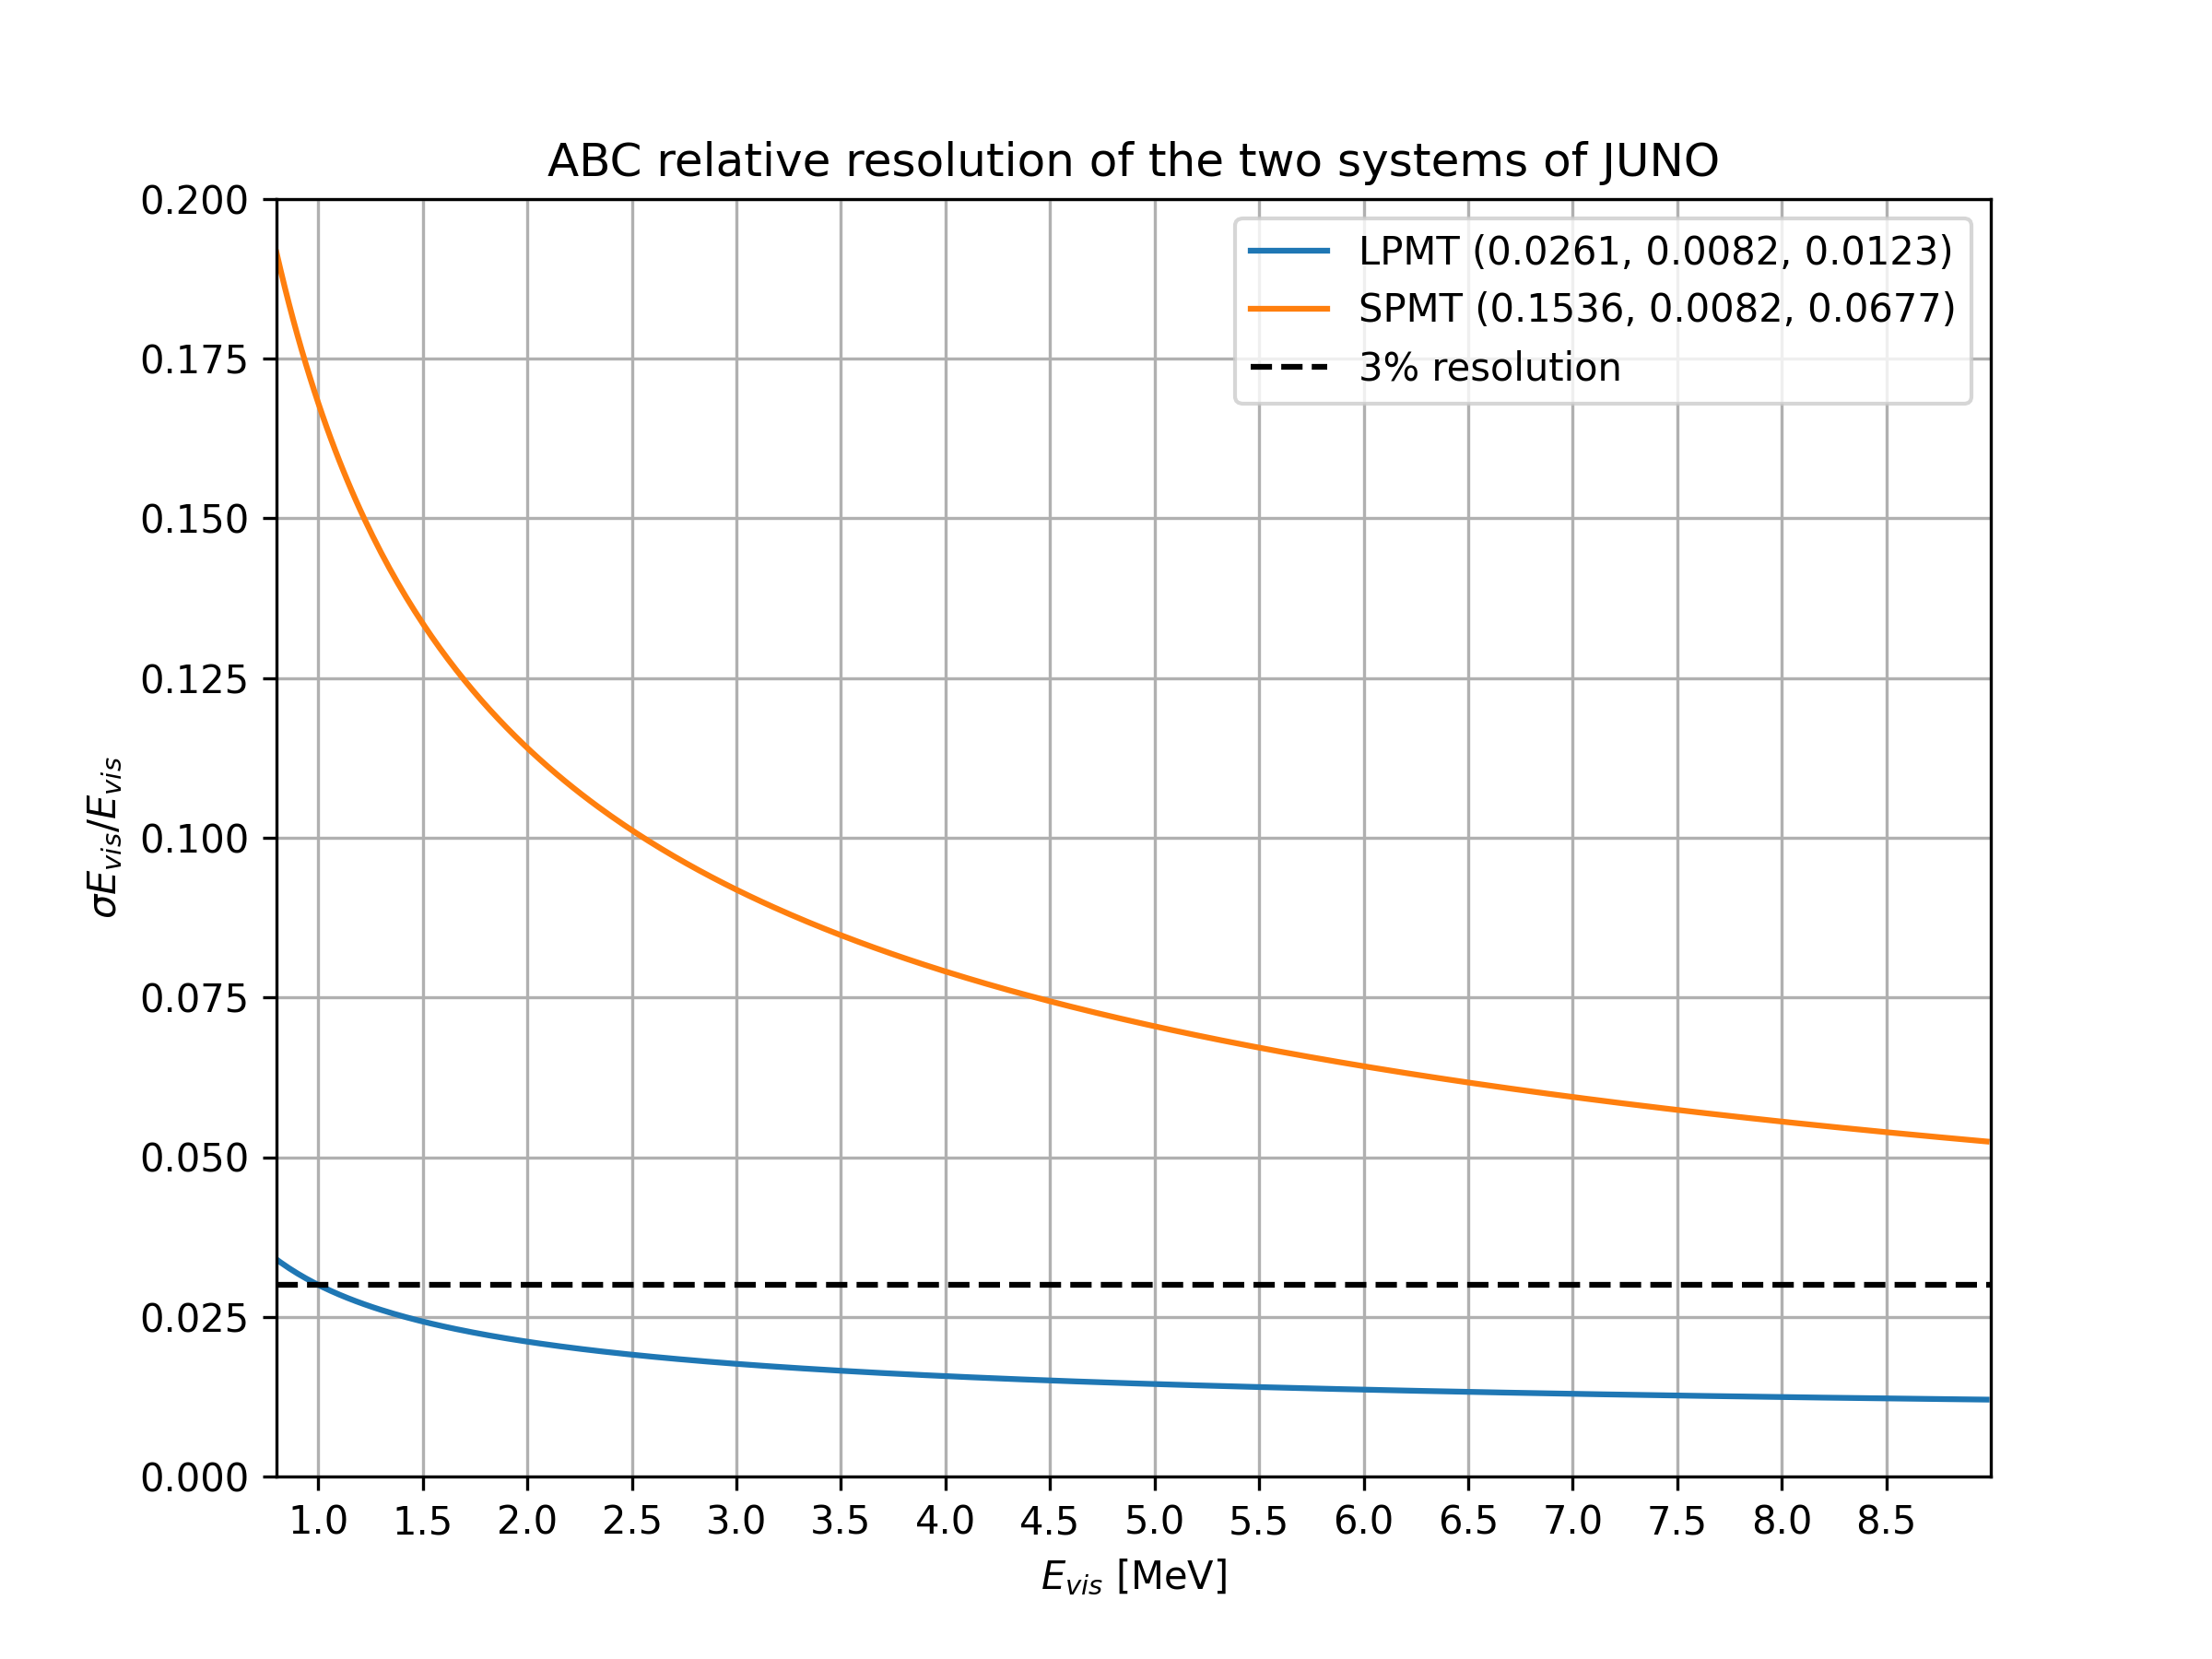
\includegraphics[width=\linewidth]{scripts/plots/relative_resolution.png}
  \end{subfigure}
  \hfill
  \begin{subfigure}[t]{0.48\linewidth}
    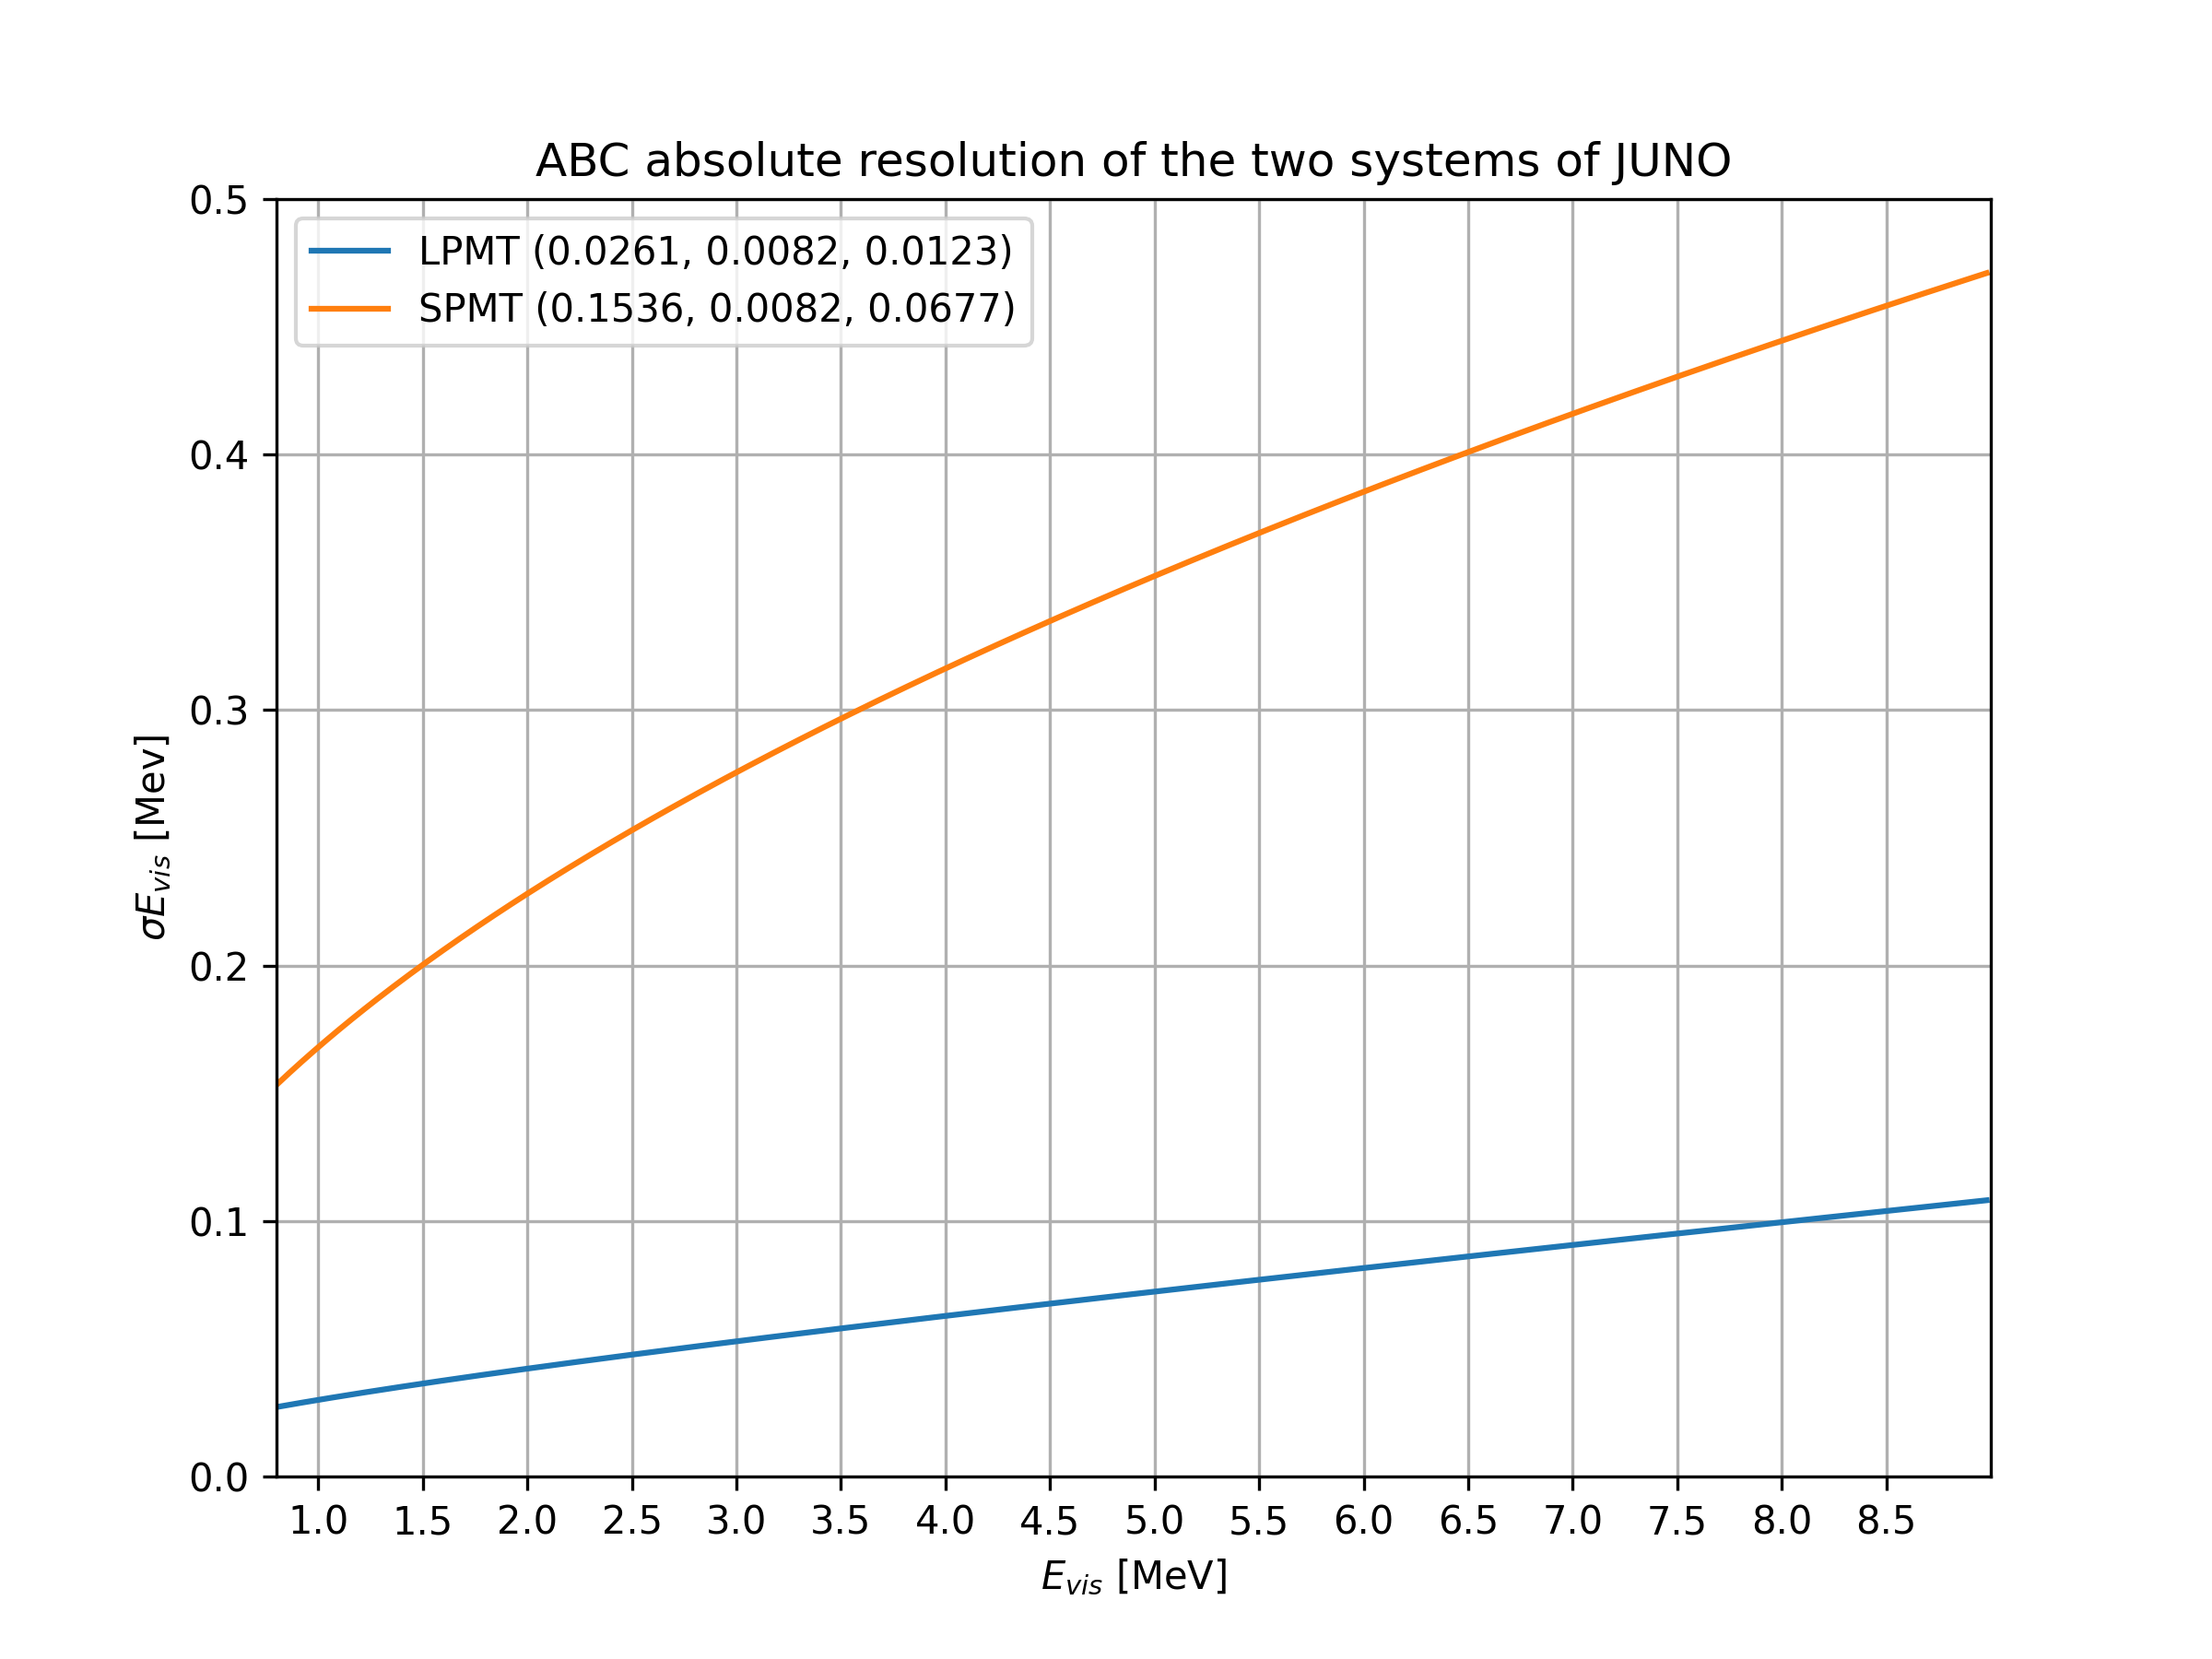
\includegraphics[width=\linewidth]{scripts/plots/absolute_resolution.png}
  \end{subfigure}
  \caption{Relative (\textbf{On the left}) and absolute (\textbf{On the right}) resolutions of the LPMT and SPMT systems used in this study. The number in parenthesis are the parameter $A$, $B$ and $C$ respectively for each systems.}
  \label{fig:joint_fit:system_resolution}
\end{figure}

%
%   (c) Le framework de fit intégré.

\subsection{Fit}
\label{sec:joint_fit:framework:fit}

The fit macro is the core of this fitting procedure. This macro is responsible for loading the fit configuration and setup the Avenue framework. Using Avenue, it will setup the data files, theoretical spectrum, choose the binning, $\chi^2$, etc... It also have the possibility to generate toys on the fly based on the theoretical spectrum. Given this theoretical spectrum we can randomize the bin content either by:
\begin{enumerate}
  \item Drawing the bin content in a Poisson distribution with the bin content as parameter.
  \item Drawing the bin content in a Gaussian distribution with the bin content as mean and variance. The bin content is then rounded to the nearest integer.
  \item Drawing the bin difference following a given covariance matrix using the Choleski decomposition. This matrix is at least the statistical covariance matrix but can also contain systematic uncertainties.
    \begin{align}
      V &= LL^T \\
      \mathbf{R} &\sim \mathcal{N}(0, 1) \\
      \tilde{\mathbf{h}} &= \lceil \mathbf{h} + L\mathbf{R} \rfloor \\
    \end{align}
    where $V$ is covariance matrix used to produce the fluctuations, $\mathbf{R}$ is drawn in a multinomal distribution of mean 0 and variance 1, $\mathbf{h}$ the bin content of the theoretical spectrum and $\tilde{\mathbf{h}}$ the bin content of the generated toy.
\end{enumerate}

The first two methods allow for the fast production of independent toys while the third allow for the production of statistical and systematical dependent toys. Unfortunately, none of those methods are fitted to produce toy with a QNL different from the theoretical spectrum. The uncertainty on the reconstructed energy $\sigma E_{rec}$ being dependent on $E_{vis}/E_{\alpha}$ makes that we would need to deconvolute the reconstruction effect from the theoretical spectrum. It is much easier to just produce those toys from the IBD generator.

% V) Tes développements techniques.
% -----------------------------------------------------------
%
%   (a) Pour générer les divers toys et pdf dont on a besoin, avec ou sans QNL.
%      --- Bien préciser les deux façons de générer des toys : dans IBDgen, ou dans le fmwk intégré, à partir de la matrice de corr et de Choleski.
%
%    (b)  Pour que le framework intégré soit capable de faire un fit joint.
%
% À ce stade, le lecteur doit comprendre comment tout est fait en pratique, et réaliser la quantité de travail technique que cela a demandé.
\section{Technical challenges and development}
\label{sec:joint_fit:tech}

The fit framework Avenue was already partially developed with multispectra fitting in mind but a lot technical development was necessary to allow for a joint fit. The first step was to migrate the framework from ROOT5 (last release in March 2018) to ROOT6 (v6.26.06 released in July 2022) to ensure compatibility with the data coming from the JUNO collaboration, and benefiting of the improvement and corrections that came with ROOT6. This allow us to upgrade the C++ standard from C++11 to C++17. A substantial effort has been done to modernize the code, generalizing the functions and methods via templating to help readability and using smart pointer to prevent possible memory leaks.

The Avenue framework had to be adapted, notably on the chi-square calculation and spectrum generation to correctly take into account the correlation between the SPMT and LPMT spectra. The delta joint fit requiring two more parameters over a spectrum twice as large as before with LPMT takes much more time, around 15h for 6 years exposure, than the single LPMT fit. Thus the framework and the fit macro had to be updated for distributed computing. Notably the aggregation of fit results can now be done in a single file instead of managing a file per fit. In case of numerous toy, the hard drive access time could lead to long analysis time.

While the IBD generator was already able to generate LPMT and SPMT spectrum, it was not designed for generating correlated spectrum. As detailed in section \ref{sec:joint_fit:framework:ibd-gen}, up to the reconstruction effect, the two spectrum need to share the same generation else the two spectrum would be decorrelated and it would be like we would run two different experiment.

\section{Results}
\label{sec:joint_fit:results}
% VI) Résultats
% ----------------------
%
%    (a) Validations techniques.
%
%        i- Les test Asimov sans QNL que nous avions faits, pour valider que le fit joint est OK techniquement (joint vs. Moyenne pondérée des fit individuels) et notamment que la matrice a été mise correctement.
%
%        ii- Tous les autres que je n'ai plus en tête.

\subsection{Validation}
\label{sec:joint_fit:validation}

The first step is to confirm that the updated fit framework is able to reproduce existing results and that the joint fit behave as expected, meaning
\begin{itemize}
  \item Without QNL, the individual (\textit{LPMT} and \textit{SPMT}) fit converge to the parameters nominal values and their errors are similar to the ones reported in existing analysis such as \cite{juno_collaboration_sub-percent_2022}.
  \item The standard joint fit with an independent covariance matrix (\textit{Indep Standard joint}), meaning that the covariance between the LPMT and SPMT spectra is 0, believe to have twice as much informations, and thus believe to have a grater precision than the individual fits.
  \item The standard joint (\textit{Standard joint}) fit with a correlated covariance matrix has errors similar to the LPMT individual fit as the LPMT drive the precision on $\theta_{13}$ and $\Delta m^2_{31}$ and that the LPMT as SPMT are expected to have close precision on $\theta_{12}$ and $\Delta m^2_{21}$.
  \item The delta joint (\textit{Delta joint}) fit with covariance matrix have the same resolution as the standard joint fit. The supplementary parameter $\delta \theta_{12}$ and $\delta \Delta m^2_{21}$ should not bring supplementary precision.
\end{itemize}

The italicized name are the name used in the results reports to identify each fit. We also look into the \textit{Indep Delta joint}, which is the Delta Joint fit but the covariance between the LPMT and SPMT spectra is 0, and the \textit{Weighted} results where
\begin{equation}
  \frac{1}{\sigma^2_{Weighted}} = \frac{1}{\sigma^2_{LPMT}} + \frac{1}{\sigma^2_{SPMT}}
\end{equation}
We expect the weighted resolution to be similar to the \textit{Indep Standard joint} as, in both of those test, we do not consider the correlation between the SPMT and LPMT results.

\subsubsection{Asimov studies}

We ran Asimov studies on the tests presented above on the updated framework, the results are reported in table \ref{tab:joint_fit:asimov_results}. All those test are ran considering statistics error only, 6 years exposure with all backgrounds, Pearson $\chi^2$ (covariance is estimated using data spectrum) and $\theta_{13}$ fixed to nominal value. For the \textit{SPMT} fit $\Delta m^2_{31}$ is fixed at nominal value as the SPMT system is net expected to be sensitive to this parameter.

\begin{table}[ht]
  \begin{footnotesize}
  \centering
  \begin{tabular}{l | c | c | c | c | c | c }
                                    & $\Delta m^2_{21}$ error  & $\delta \Delta m^2_{21}$ error & $\theta_{12}$ error   & $\delta \theta_{12}$ error  & $\Delta m^2_{31}$ error & $\chi^2$ \\
                                    \hline
  LPMT                                 & 1.29936e-07   &               & 1.33852e-03   &               & 4.39399e-06   & 3.23088e-18 \\
  SPMT                                 & 1.38297e-07   &               & 1.38653e-03   &               &               & 2.87502e-18 \\
  Indep Standard joint                 & 9.48731e-08   &               & 9.86765e-04   &               & 4.39212e-06   & 6.10592e-18 \\
  Standard joint                       & 1.29723e-07   &               & 1.18342e-03   &               & 4.39287e-06   & 3.38055e-18 \\
  Weighted                             & 9.46966e-08   &               & 9.63002e-04   &               &               & \\
  \hline
  Delta joint                            & 1.35780e-07   & 3.43529e-08   & 1.38236e-03   & 1.46865e-04   & 4.39309e-06   & 3.38055e-18 \\
  Indep Delta joint                      & 1.38297e-07   & 1.89391e-07   & 1.38653e-03   & 1.87830e-03   & 4.39241e-06   & 6.10592e-18 \\
  \hline
  \hline
  \multicolumn{7}{c}{Fixed $\Delta m^2_{21}$ and $\Delta m^2_{31}$} \\
  \hline
  Indep Standard joint &               &               & 9.33082e-04   &               &               & 4.82955e-26 \\
  LPMT                 &               &               & 1.27032e-03   &               &               & 2.58849e-26 \\
  SMPT                 &               &               & 1.31070e-03   &               &               & 2.24106e-26 \\
  Weighted             &               &               & 9.12193e-04   &               &               & \\
  \hline
  \hline
  \multicolumn{7}{c}{Fixed $\Delta m^2_{31}$ and $\theta_{12}$} \\
  \hline
  Indep Standard joint          & 8.97117e-08   &               &               &               &               & 6.10617e-18 \\
  SPMT                          & 1.30734e-07   &               &               &               &               & 2.87522e-18 \\
  LPMT                          & 1.23319e-07   &               &               &               &               & 3.23095e-18 \\
  Weighted                      & 8.97066e-08   &               &               &               &               & \\
  \end{tabular}
  \end{footnotesize}
  \caption{Results of the Asimov studies on the updated framework. All results are Asimov fit, considering 6 years exposure, $\theta_{13}$ is fixed to nominal value, $\chi^2$ is pearson meaning that he error is estimated using the data spectrum}
  \label{tab:joint_fit:asimov_results}

\end{table}

In every cases presented above, the fit converges to the parameters nominal value thus only the errors are presented.

We observe, as expected, that $\sigma_{Weighted} \approx \sigma_{Indep~Standard~joint}$ with the exception of $\sigma \theta_{12}$. This could from the slight difference in statistic between the SPMT and LPMT spectra. Indeed, due to a larger smearing in energy resolution, events that would be inside the spectrum range [0.8, 7.5] MeV are smeared outside it. This deficit is partially compensated by event outside the spectrum coming back in it but we expect very few event outside the spectrum in comparison to event at the edges of it. Thus the event deficit is not totally compensated. $\theta_{12}$ being mainly driven by the amplitude of the spectrum (see illustration \ref{fig:juno:juno-spectrum-oscillation}), that's why we think this the origin of the difference.

The second observation is that $\sigma_{Standard~joint} \approx \sigma_{LPMT}$. Once the covariance matrix between the LPMT and SPMT is correctly introduced, the fit ``understand'' that it does not have supplementary information and the LPMT system, which have the best precision, dominate the resolution.

Finally for the \textit{Delta} fit, the error on $\delta \theta_{12}$ and $\delta \Delta m^2_{21}$ are of the same order of magnitude than the errors on $\theta_{12}$ and $\Delta m^2_{21}$ in the absence of the covariance matrix. As the LPMT and SPMT spectra are not connected through the covariance matrix, the delta parameters are unconstrained thus the similar errors. Once the covariance matrix is introduced, the delta are much more constrained and show errors of an order of magnitude smaller than the error on their respective parameters.

Overall, the asimov studies are satisfactory. The joint fit behave as expected and the errors on the delta parameters are significantly smaller than the error on their respective parameters, indicating great potential if they converge to value too far from 0.

\subsubsection{Toy studies}

Once we validated that the asimov study is yielding coherent results, we study the behaviour of toy studies. The above asimov study was using the Pearson $\chi^2$ (Eq. \ref{eq:joint_fit:pearson}) without pull parameter. We show in figure \ref{fig:joint_fit:abs_standard_pearson} the effect of using a simple Pearson $\chi^2$. We see that $\sin^2(2\theta_{12})$ (reported as $\theta_{12}$ for simplicity) is biased of about $0.5\sigma$ and $\Delta m^2_{21}$ biased of about $0.1\sigma$. When introducing the PearsonV $\chi^2$ (Eq. \ref{eq:joint_fit:pearsonV}) the bias disappear as reported in figure \ref{fig:joint_fit:abs_standard_pearsonV}.

\begin{figure}[ht]
  \centering
  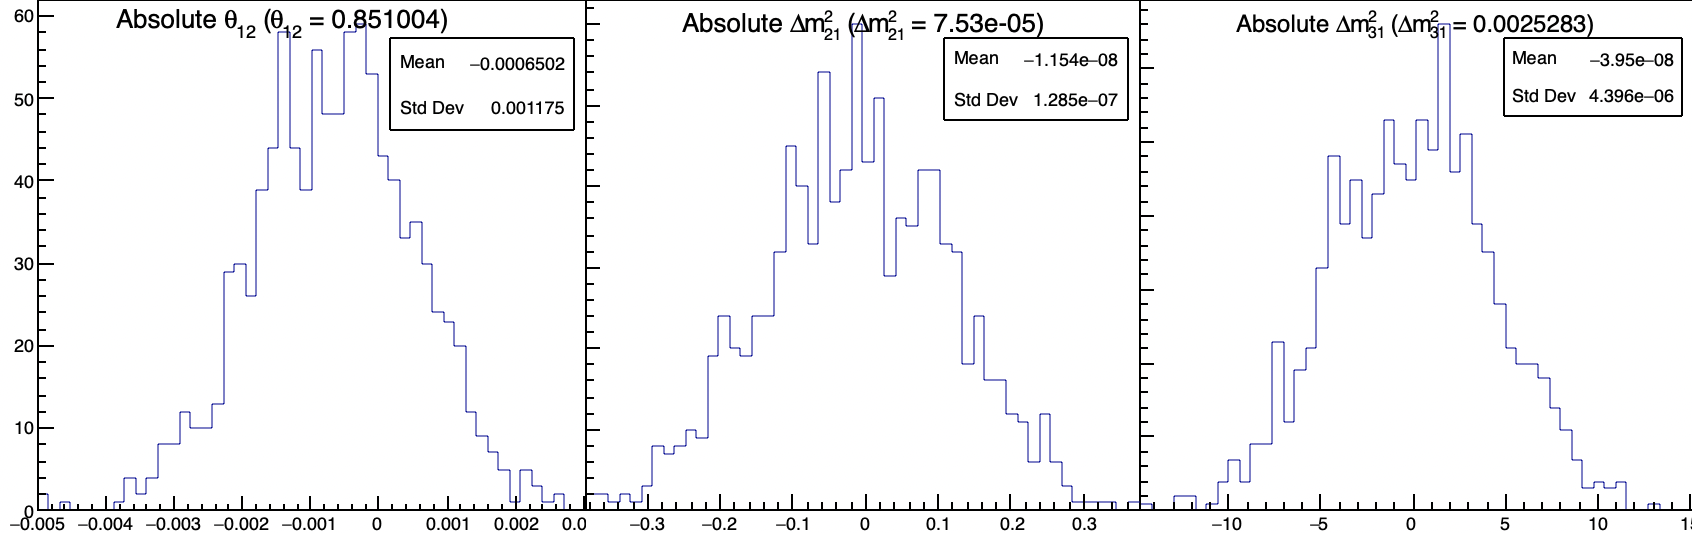
\includegraphics[width=\linewidth]{images/joint_fit/absolute_standard_joint_pearson.png}
  \caption{Distribution of BFP - nominal value for 1000 toy Standard joint fit. 6 years exposure, all background, \textbf{Pearson} $\chi^2$, $\theta_{13}$ fixed.}
  \label{fig:joint_fit:abs_standard_pearson}
\end{figure}

\begin{figure}[ht]
  \centering
  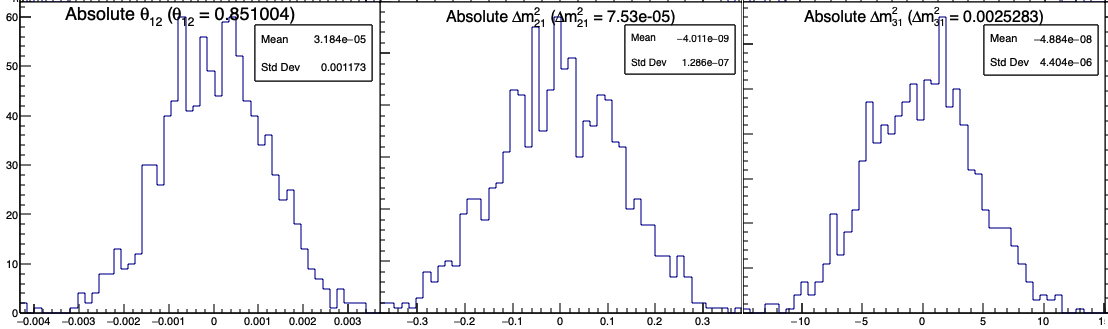
\includegraphics[width=\linewidth]{images/joint_fit/absolute_standard_joint_pearsonV.png}
  \caption{Distribution of BFP - nominal value for 1000 toy Standard joint fit. 6 years exposure, all background, \textbf{PearsonV} $\chi^2$, $\theta_{13}$ fixed.}
  \label{fig:joint_fit:abs_standard_pearsonV}
\end{figure}

When the supplementary parameters are introduced in the Delta Joint fit, the fit is stable as shown in the results figure \ref{fig:joint_fit:delta_fit}. The resolutions on the oscillation parameters are slightly worse in the Delta joint fit due to the supplementary freedom. As seen in the asimov studies, the resolution of the $\delta$ parameters is an order of magnitude smaller than their respective parameters, indicating that they can be powerful tools to detect discrepancies between the SPMT and LPMT spectra.

\begin{figure}[ht]
  \centering
  \begin{subfigure}[t]{0.98\linewidth}
    \centering
    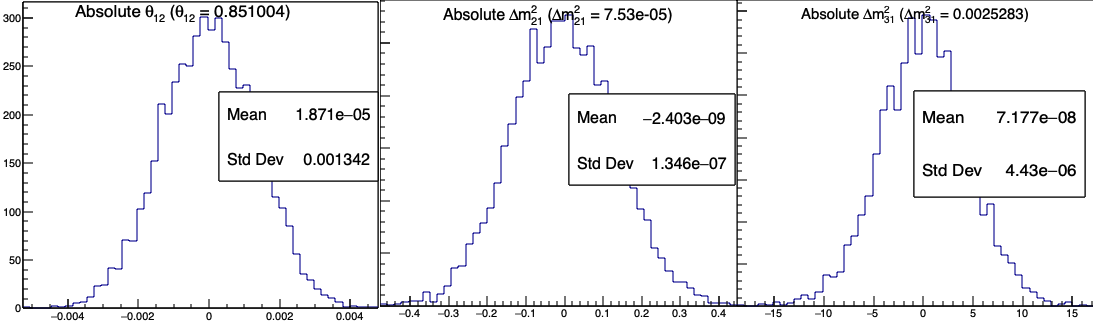
\includegraphics[width=\linewidth]{images/joint_fit/normal_delta_joint.png}
  \end{subfigure}

  \begin{subfigure}[t]{0.66\linewidth}
    \centering
    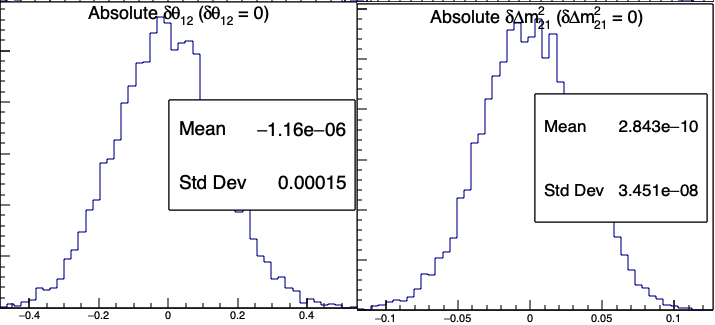
\includegraphics[width=\linewidth]{images/joint_fit/supp_delta_joint.png}
  \end{subfigure}

  \caption{Distribution of BFP - nominal value for 5000 toy Delta joint fit. 6 years exposure, all background, \textbf{PearsonV} $\chi^2$, $\theta_{13}$ fixed.}
  \label{fig:joint_fit:delta_fit}
\end{figure}

\subsubsection{Effect of supplementary QNL on the LPMT spectrum}

Now that we know that the framework and joint fit behave correctly on unbiased data, we test the effect of introducing the QNL, as presented in Eq. \ref{eq:joint_fit:alpha_yang}, in the LPMT spectrum. To test the effect, we consider a QNL $\alpha_{qnl} = 1\%$. For reference, this is about three time the expected residual QNL after calibration ($\alpha_{qnl} = 0.3\%$ \cite{juno_collaboration_calibration_2021}). The background had to be removed as JUNO provide them already smeared, thus the introduction of supplementary QNL is not trivial, the resolution being dependent of $E_{vis}$ which is affected by the QNL.
We use a covariance matrix assuming no QNL. The effect of this QNL on the spectrum is illustrated in figure \ref{fig:joint_fit:anom_aqnl}. In table \ref{tab:joint_fit:qnl_results} we report the results of the different scenarios.

\begin{figure}[ht]
  \centering
  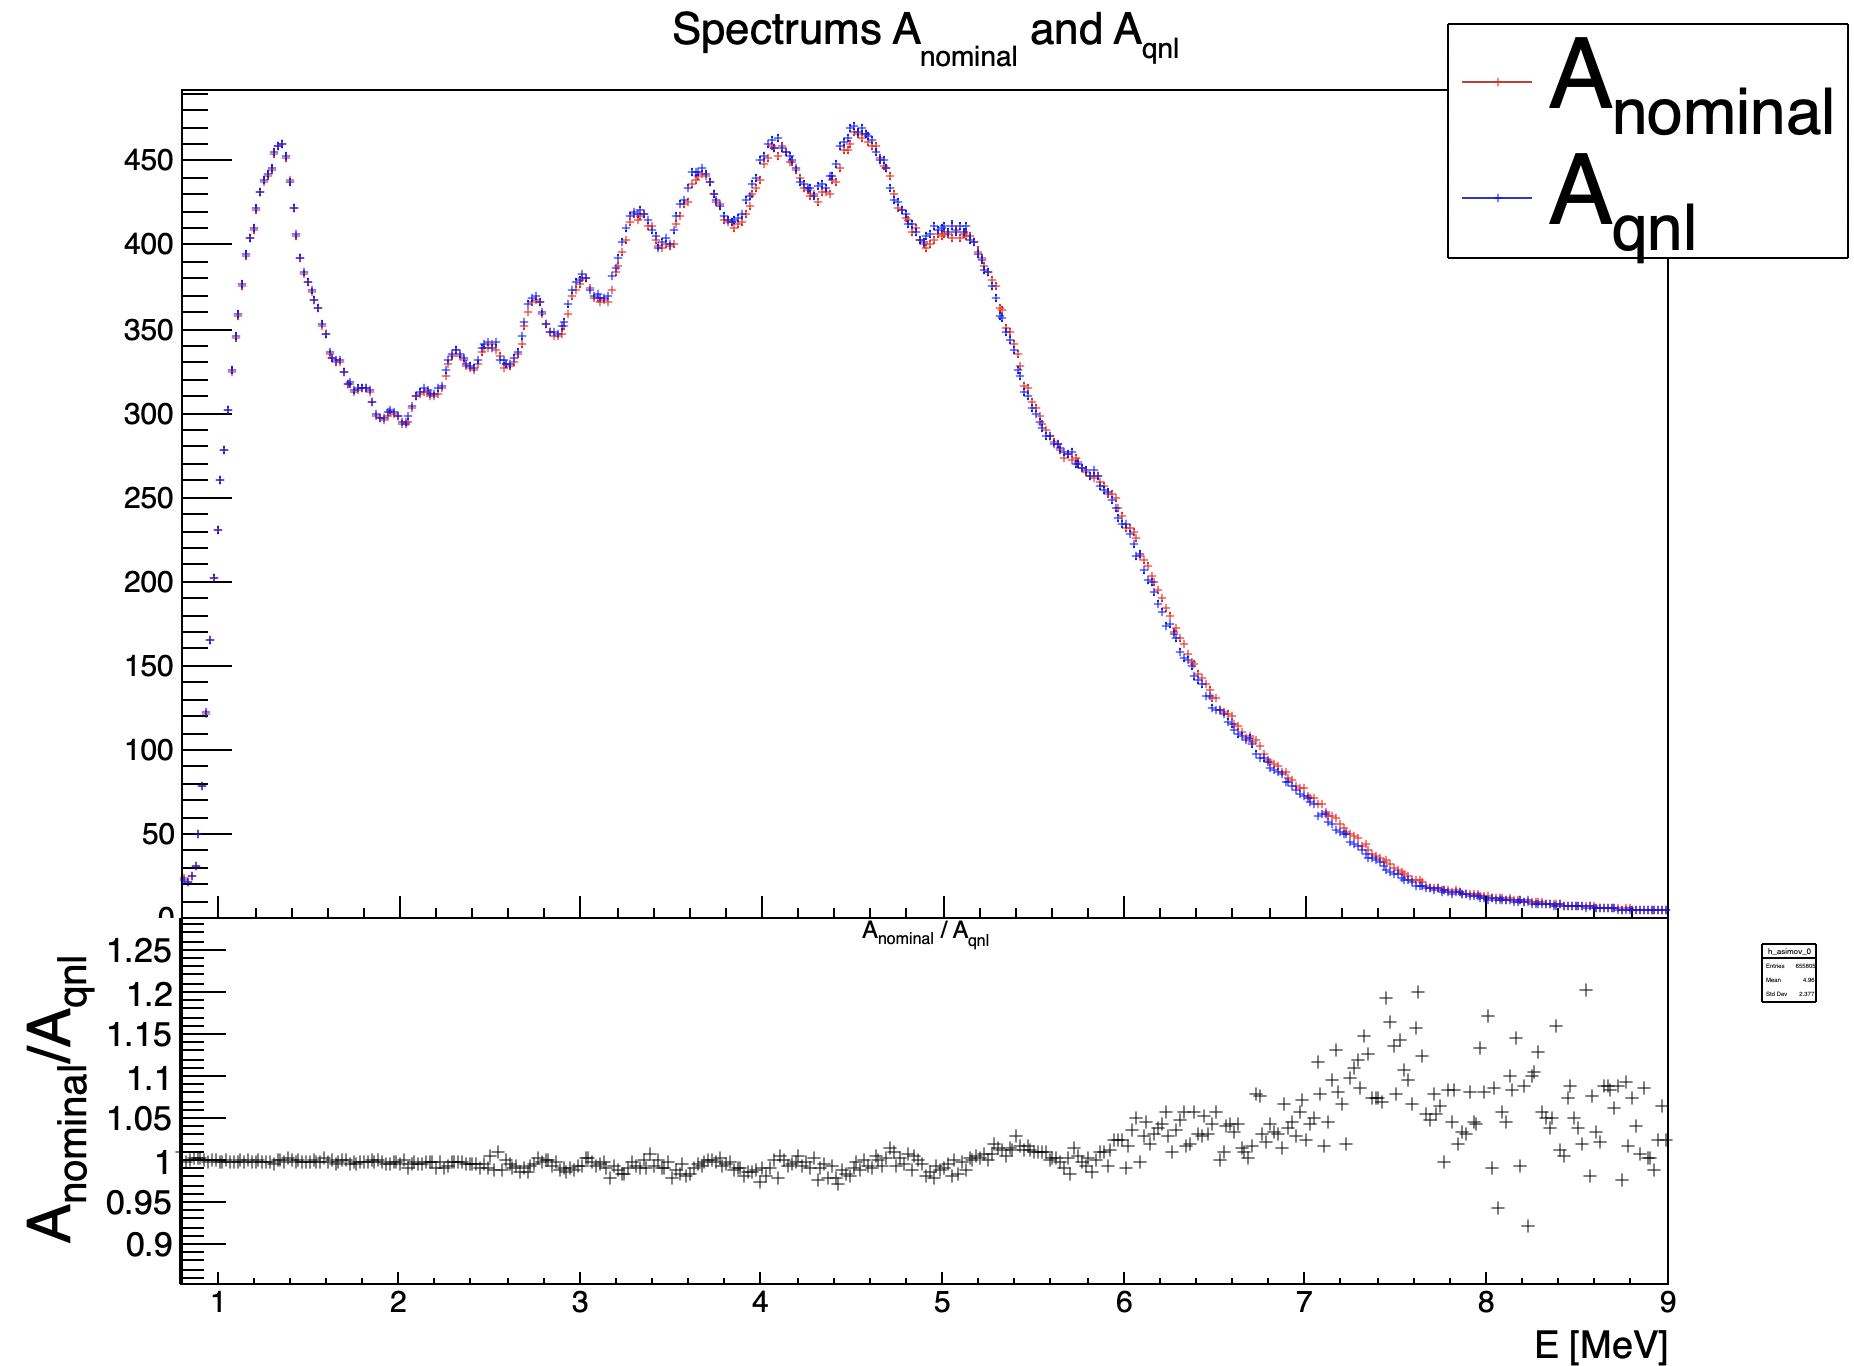
\includegraphics[height=6cm]{images/joint_fit/AnominalAQNL.png}
  \caption{\textbf{Top:} Theoretical spectrum without QNL (in red) and with $\alpha_{qnl} = 1\%$ (in blue). \textbf{Bottom:} Ratio between the theoretical spectrum with and without QNL.}
  \label{fig:joint_fit:anom_aqnl}
\end{figure}



\begin{table}[h]
  \begin{footnotesize}
  \centering
  \begin{tabular}{l|lr|lr|lr|lr|lr|}
    Mean (std dev)  & \multicolumn{2}{c|}{$\theta_{12}$ [$10^{-3}$]} & \multicolumn{2}{c|}{$\Delta m^2_{21}$ [$10^{-7}\mathrm{eV}^{2}$]} & \multicolumn{2}{c|}{$\Delta m^2_{31}$ [$10^{-6}\mathrm{eV}^{2}$]} & \multicolumn{2}{c|}{$\delta \theta_{12}$ [$10^{-3}$]} & \multicolumn{2}{c|}{$\delta \Delta m^2_{21}$ [$10^{-7}\mathrm{eV}^{2}$]} \\
    \hline
    LPMT            & -1.569 & (1.171) & -0.957 & (0.989) & -8.235 & (3.898)       & \multicolumn{2}{c|}{Irrelevant} & \multicolumn{2}{c|}{Irrelevant}  \\
    SPMT            & -0.164 & (1.191) & -0.603 & (1.054) & \multicolumn{2}{c|}{Not sensitive} &\multicolumn{2}{c|}{Irrelevant} & \multicolumn{2}{c|}{Irrelevant}  \\
    Indep Standard  & -0.880 & (1.174) & -0.786 & (1.004) & -8.195 & (3.900)       & \multicolumn{2}{c|}{Irrelevant} & \multicolumn{2}{c|}{Irrelevant}  \\
    Standard        & -8.106 & (1.423) & -2.483 & (1.018) & -6.649 & (4.008)       & \multicolumn{2}{c|}{Irrelevant} & \multicolumn{2}{c|}{Irrelevant}  \\
    Indep Delta     & -0.169 & (1.190) & -0.598 & (1.054) & -8.234 & (3.899)       & -1.397 & (0.259)     & -0.361 & (0.366) \\
    Delta           & -0.163 & (1.183) & -1.532 & (1.036) & -8.193 & (3.934)       & -1.441 & (0.193)     & 0.654  & (0.303) \\
  \end{tabular}
  \end{footnotesize}
  \caption{Results of the different fit scenarios on QNL distorted data $\alpha_{qnl} = 1\%$. The mean value are reported subtracted from their nominal value. For SPMT $\Delta m^2_{31}$ is fixed at nominal value. The $\chi^2$ is PearsonV. The correlation matrix used to fit assume no QNL in the spectrum.}
  \label{tab:joint_fit:qnl_results}
\end{table}

The results in table \ref{tab:joint_fit:qnl_results} are subtracted from their nominal value, themselves reported in table \ref{tab:joint_fit:pdg_value}. We clearly see the bias induced by $\alpha_{qnl} = 1\%$ when comparing the SPMT and LPMT results. The Indep Standard is, as expected, the mean value between the SPMT and LPMT: the fit having no informations about the correlation between the spectrum think it have two uncorrelated experiments thus report an in between value. When introducing the relationship between the LPMT and SPMT spectra in the Standard fit, the joint fit cannot find a clean minima, it thus converge to a completely incorrect value.

Introducing the $\delta$ without the correlation in Delta Indep remove the bias and converge to the SPMT minima, the $\delta$ absorbing the deformation of the LPMT spectra.

Finally, with the $\delta$ and the covariance matrix, $\theta_{12}$ is unbiased, $\delta \theta_{12}$ absorbing the deformation. $\delta \Delta m^2_{21}$ is still heavily biased, even more than LPMT only, for the same reason than the Standard fit: the correlation make it difficult to converge to the nominal value.

Overall $\Delta m^2_{31}$ bias is unchanged as the SPMT spectrum bring no information about the parameter. The $\delta$ are significant, naively up to 7.46$\sigma$ for $\delta \theta_{12}$ in the Delta fit.




%   (b) La matrice de covariance
%
%      i- méthode théorique
%         --- explications
%         --- résultats
%      ii- méthode toys
%             Idem
%      iii- la méthode basée sur les données sniper.
%            Idem
%      iv- comparaison
%         --- commentaires et conclusion.
%
%     Préciser ou rappeler ici que
%         --- pour nos tests, nous nous basons sur l'hypo H0 et donc nous générons la matrice sans QNL.
%         --- les corrélations dépendent peu de la forme du spectre ou se sa stat.
\subsection{Covariance matrix}
\label{sec:joint_fit:cov_mat}

The covariance matrix between the LPMT and SPMT spectra is at the hearth of this study as it was already mentioned in section \ref{sec:joint_fit:approach} and demonstrated in section \ref{sec:joint_fit:validation}. In this section we discuss the different approaches taken to estimate it. In this work we will mainly discuss the statistical covariance matrix between the two spectra, how the number of event in a LPMT bin influence the number of bin in the SPMT spectrim due to the resolution. We will still discuss the reconstruction effects, mostly due to non-uniformity, in on reconstruction correlation.

\subsubsection{Analytical method}

The first method discussed is the analytical method where we propagate the resolution of the LPMT and SPMT spectra over a non-smeared spectrum. Following the approach used in the IBD generation in section \ref{sec:joint_fit:framework:ibd-gen}, we consider the system resolution $\sigma(E)$ to be only dependent in energy. We do not consider the position of the event.

The first step is to compute the statistical uncertainty of the input spectrum while taking into account the smearing, considering no uncertainty on the smearing. For this, using the notation of section \textit{39.2.5 Propagation of errors} of PDG2020 \cite{particle_data_group_review_2020} and considering an extended spectrum of 820 bins following the binning scheme introduced in \ref{sec:joint_fit:data_gen}, the first 410 for the LPMT and the last 410, we consider
\begin{itemize}
  \item $\bm{\theta} = (\theta_0, ..., \theta_n);~ n = 820$ the content of the spectrum bins.
  \item $\bm{\eta}(\bm{\theta}) = (\eta_0(\bm{\theta}), ..., \eta_m(\bm{\theta})); ~ m  = 820$ the set of smearing functions representing the PMT resolutions.
\end{itemize}

$\eta_m$ can thus be defined as
\begin{equation}
  \label{eq:joint_fit:cov_ana:eta}
  \eta_i  = \sum_j^n G(i, \sigma(E_i))(j) \theta_j
\end{equation}
where $G(i, \sigma(E_i))(j)$ is the smearing function defined as
\begin{equation}
  G(i, \sigma(E_i))(j) = \int_{\lfloor E_j\rfloor}^{\lceil E_j \rceil} \frac{1}{\sigma(E_i)\sqrt{2\pi}} e^{-\frac{(E_i-E)^2}{2\sigma(E_i)^2}} \dd{E}
\end{equation}
where $E_i$ is the mean energy in the bin $i$ and $\lfloor E_i\rfloor$ and $\lceil E_i \rceil$ are the lower and higher energy bound of the $i$th bin respectively.

We can then construct the transfer matrix $A$ as
\begin{equation}
  A_{ij} = \frac{\partial\eta_i}{\partial\theta_j} = G(i, \sigma(E_i))(j)
\end{equation}
and then compute the first part of our covariance matrix
\begin{equation}
  U = AVA^T
\end{equation}
where $V$ is the uncorrelated covariance matrix simply defined, under the assumption of poissonian statistic for the bin content,
\begin{equation}
  V_{ij} = \sqrt{\theta_i \theta_j}
\end{equation}

Now we just need to consider the uncertainty on the smearing $\sigma \eta_i$, considering no uncertainty on the unsmeared spectrum. From Eq. \ref{eq:joint_fit:cov_ana:eta}, the $G(i, j) \equiv G(i, \sigma(E_i))(j)$ are considered independents from each other $\forall i, j$. This mean that this covariance matrix is diagonal, we only need $\sigma G(i, j)$. We can derive this term from two equation:
\begin{itemize}
  \item The term $G(i, j)\theta_j$ represent the number of event smeared from the bin $j$ that end up in the bin $i$. This is a number, we thus assume poissonian statistic so that $\sigma[G(i, j)\theta_j] = \sqrt{G(i, j) \theta_k}$.
  \item Using basic error propagation we can say that $\sigma^2[G(i, j)\theta_j] =\theta_j^2 \sigma^2G(i, j) + G(i, j)^2 \sigma^2 \theta_j$.
\end{itemize}
Using $\sigma\theta_j = \sqrt{\theta_j}$ we derive
\begin{align}
  G(i, j) \theta_j &= \sigma^2[G(i, j)\theta_j] =\theta_j^2 \sigma^2G(i, j) + G(i, j)^2 \theta_j \\
  \Rrightarrow \sigma^2 G(i, j) &= \frac{G(i, j) \theta_j - G(i, j)^2 \theta_j}{\theta_j^2} \\
                                &= \frac{(1 - G(i, j))G(i, j)}{\theta_j}
\end{align}

By summing the two covariance matrix, we can extract a correlation matrix presented in figure \ref{fig:joint_fit:th_cor_mat}. The correlation between the SPMT and LPMT spectra is greater at the start of the spectrum, where the absolute smearing is the smallest, up to 5\% correlation, and diffuse as the bins are further from each other and the absolute resolution grow.

\begin{figure}[ht]
  \centering
  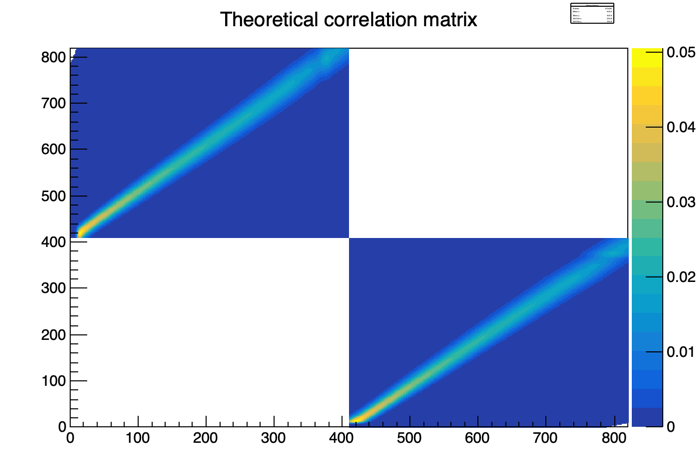
\includegraphics[height=6cm]{images/joint_fit/theoretical_corr.png}
  \caption{Theoretical correlation matrix between the LPMT spectrum (bins 0-409) ans the SPMT spectrum (410-819). The diagonal has been set to 0 (it was 1) for readability purpose.}
  \label{fig:joint_fit:th_cor_mat}
\end{figure}

\subsubsection{Empiric method}

The second method is the empric way where we generate toys and just compute the empirical correlation between the bin contents.
\begin{equation}
  \mathrm{Corr}(\theta_i, \theta_j) = \frac{\mathbb{E}[\theta_i \theta_j] - \mathbb{E}[\theta_i] \mathbb{E}[\theta_j]}{\sigma \theta_i \sigma \theta_j}
\end{equation}

We thus generate $10^7$ event using the IBD generator presented in section \ref{sec:joint_fit:framework:ibd-gen}, then produce spectra from this finite set of events, meaning we must choose a number $N$ of toy each composed of $M$ event in order to have the best estimate.

Due to the nature of our estimator, the estimated correlation coefficient is subject to statistical fluctuation as any estimator. There is no definite formula to compute the standard deviation of the correlation coefficient as suggested in this study \cite{gnambs_brief_2023} but all cited formula depend solely on the number of samples, in our case the number of toy $N$, and the correlation coefficient. This indicate that maximizing the number of toy is the right decision, even if each toy posses only one sole event.

To study this rather counter intuitive observation (How can a spectrum with only one event can be representative of the experiment ?), I present in figure \ref{fig:joint_fit:empirical_cor} the upper left corner of the estimated correlation matrix for different configurations of N and M in the limit of $10^7$ total event. Wee see in figure \ref{fig:joint_fit:empirical_cor:small} that if the toy number $N$ is too low, the statistical noise make the correlation pattern almost completely disappear, in figure \ref{fig:joint_fit:empirical_cor:medium} we see clearly the same correlation patter as in the theoretical matrix in figure \ref{fig:joint_fit:th_cor_mat}.
On the final matrix in figure \ref{fig:joint_fit:empirical_cor:cheff_kiss} the pattern is clearly visible, but we see a shade of anti-correlation around the spectrum that was not present in the theoretical correlation matrix.

\begin{figure}[ht]
  \begin{subfigure}[t]{0.33\linewidth}
    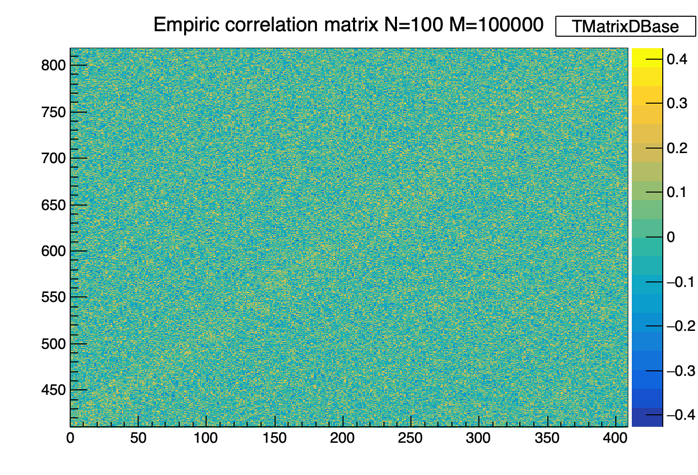
\includegraphics[width=\linewidth]{images/joint_fit/estimated_corr_N_100_M_100000.png}
    \caption{}
    \label{fig:joint_fit:empirical_cor:small}
  \end{subfigure}
  \begin{subfigure}[t]{0.33\linewidth}
    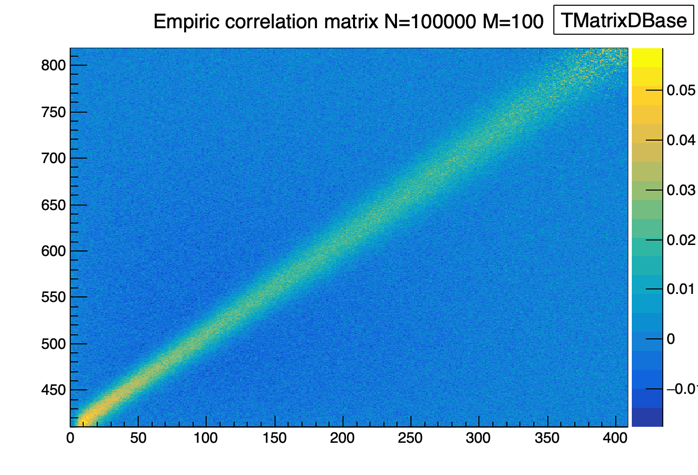
\includegraphics[width=\linewidth]{images/joint_fit/estimated_corr_N_100000_M_100.png}
    \caption{}
    \label{fig:joint_fit:empirical_cor:medium}
  \end{subfigure}
  \begin{subfigure}[t]{0.33\linewidth}
    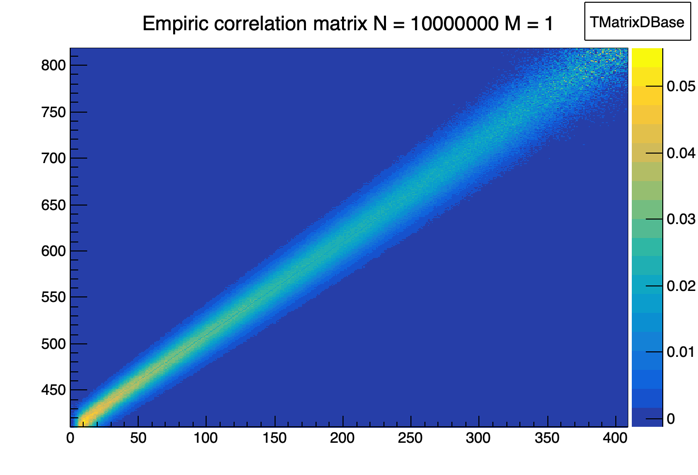
\includegraphics[width=\linewidth]{images/joint_fit/estimated_corr_N_10000000_M_1.png}
    \caption{}
    \label{fig:joint_fit:empirical_cor:cheff_kiss}
  \end{subfigure}
  \caption{Upper left corner of the estimated correlation matrix between the LPMT and SPMT spectrum for different configuration of $N$ toy with different number of $M$ events per toy}
  \label{fig:joint_fit:empirical_cor}
\end{figure}


The difference between the element of the theoretical and the empiric correlation matrices are presented in figure \ref{fig:joint_fit:th_em_diff}. We that the difference between the two is very small with a bias of $1.8 \cdot 10^{-3}$ and a standard deviation of $1.9 \cdot 10^{-3}$ while the interesting correlation are of the order $10^{-2}$. As presented in figure \ref{fig:joint_fit:th_em_diff_mat}, the most extreme differences comes from the low end of the spectrum.

This low energy difference could be explained as the theoretical does not take into account event that would be smeared from outside the spectrum. $E < 0.8$, MeV back inside the spectrum thus missing on the potential correlations.

The second major difference between the empirical and theoretical correlation matrices is the anti-correlation of magnitude $\approx -5\cdot 10^{-3}$ around the spectrum. In the theoretical correlation matrix, we assume that $G(i, j)$ is uncorrelated from $G(i, k)$ but this is not true in the case of a finite dataset. $G(i, j)$ represent the number of events that migrate from the bin $i$ to $j$, in the case of a finite number of event to distribute between the bins, the number of event that can be distributed in the bin $k$ is constrained by the number of event distributed in the bin $j$ leading to the anti-correlation between this two bins.

\begin{figure}[ht]
  \centering
  \begin{subfigure}[t]{0.49\linewidth}
    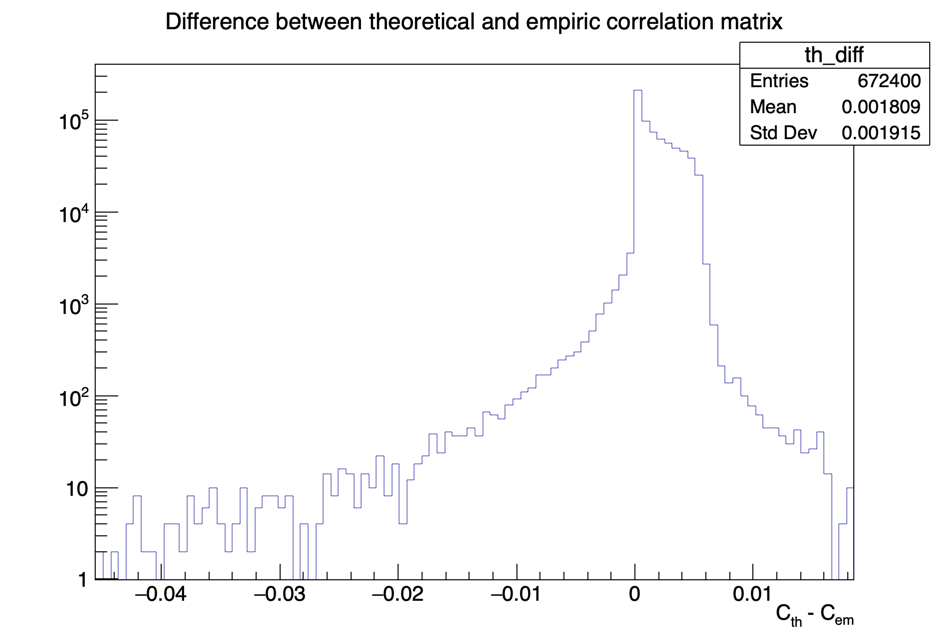
\includegraphics[width=\linewidth]{images/joint_fit/th_em_corr_diff.png}
    \caption{}
    \label{fig:joint_fit:th_em_diff}
  \end{subfigure}
  \begin{subfigure}[t]{0.49\linewidth}
    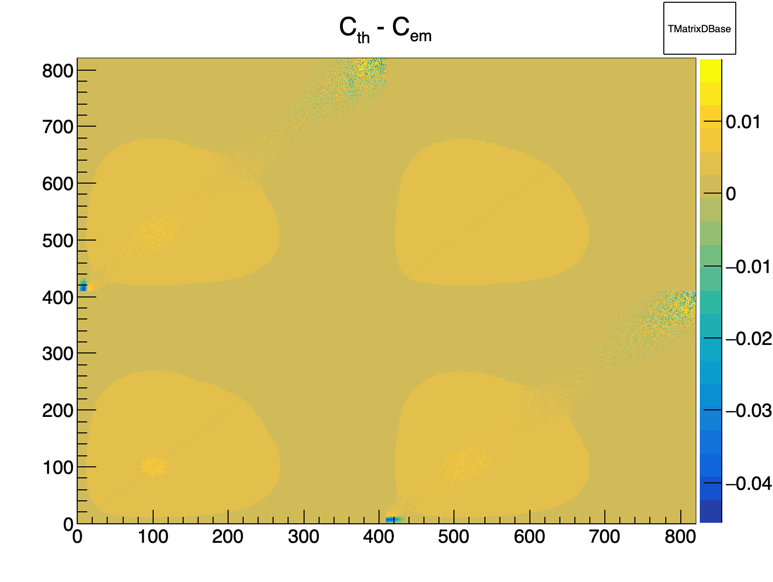
\includegraphics[width=\linewidth]{images/joint_fit/th_em_corr_diff_mat.png}
    \caption{}
    \label{fig:joint_fit:th_em_diff_mat}
  \end{subfigure}
  \caption{Difference between the element of the theoretical and empiric correlation matrix}
\end{figure}

These empirical correlation matrices still pose an issue: These matrices needs to be invertible for $\chi^2$ calculation. The framework use the Cholesky decomposition \cite{noauthor_note_1924} for this, requiring the correlation matrices to be positive definite, which is not guarantee using this empirical methods. Due to this issue, the theoretical matrix is used in the studies presented in this thesis.

\subsubsection{Empirical correlation matrix from fully simulated event}

The last study on the correlation matrix between the LPMT and SPMT spectrum consists in simulating and reconstructing full events in the official JUNO simulation framework and computing an empirical matrix based on those events.

The core of the idea is that the LPMT and SPMT reconstruction errors is bound to be correlated due to systematic effects. The first and most obvious one, for example, is energy escaping from the central detector. If the positron, or one of the two annihilation gamma, escape from the detector, less energy is deposited thus both of the systems will reconstruct a lower energy that was actually deposited. On a more subtle scale, the randomness in the production of scintillation photons is common for the two systems, if the liquid scintillator produces fewer scintillation photons for an event, both systems are likely to underestimate the energy.

We study those effects by computing from a dataset of IBD events, uniformly distributed in the CD, the correlation between the reconstruction errors on the energy
\begin{equation}
  Corr(E_{lpmt} - E_{dep}, E_{spmt} - E_{dep})
\end{equation}
where $E_{lpmt}$ and $E_{spmt}$ are the reconstructed energies from both systems and $E_{dep}$ is the deposited energy in the detector.

With this observable, the bias difference between the two reconstructions at fixed $R$ and $E$ is irrelevant. However, since we compute the correlation in $E$ and $R^3$ bins, we need to account for the potential spurious relationship between the errors and their respective biases. If the bias is small relative to the resolution, it can be ignored; but if the bias variation is on the same order of magnitude as the error, it may introduce false correlations. For this reason, based on the CNN results shown in figure \ref{fig:jcnn:vic_cnn}, we restrict our analysis to the $1 < E_{dep} < 9$ MeV range.

The results of those correlations are presented in figure \ref{fig:joint_fit:empirical_corr:E_a_R} for the single energy and radius dependency and figure \ref{fig:joint_fit:empirical_corr:E_R} for the dual energy and radius dependency.

\begin{figure}[ht]
  \centering
  \begin{subfigure}[t]{0.48\linewidth}
    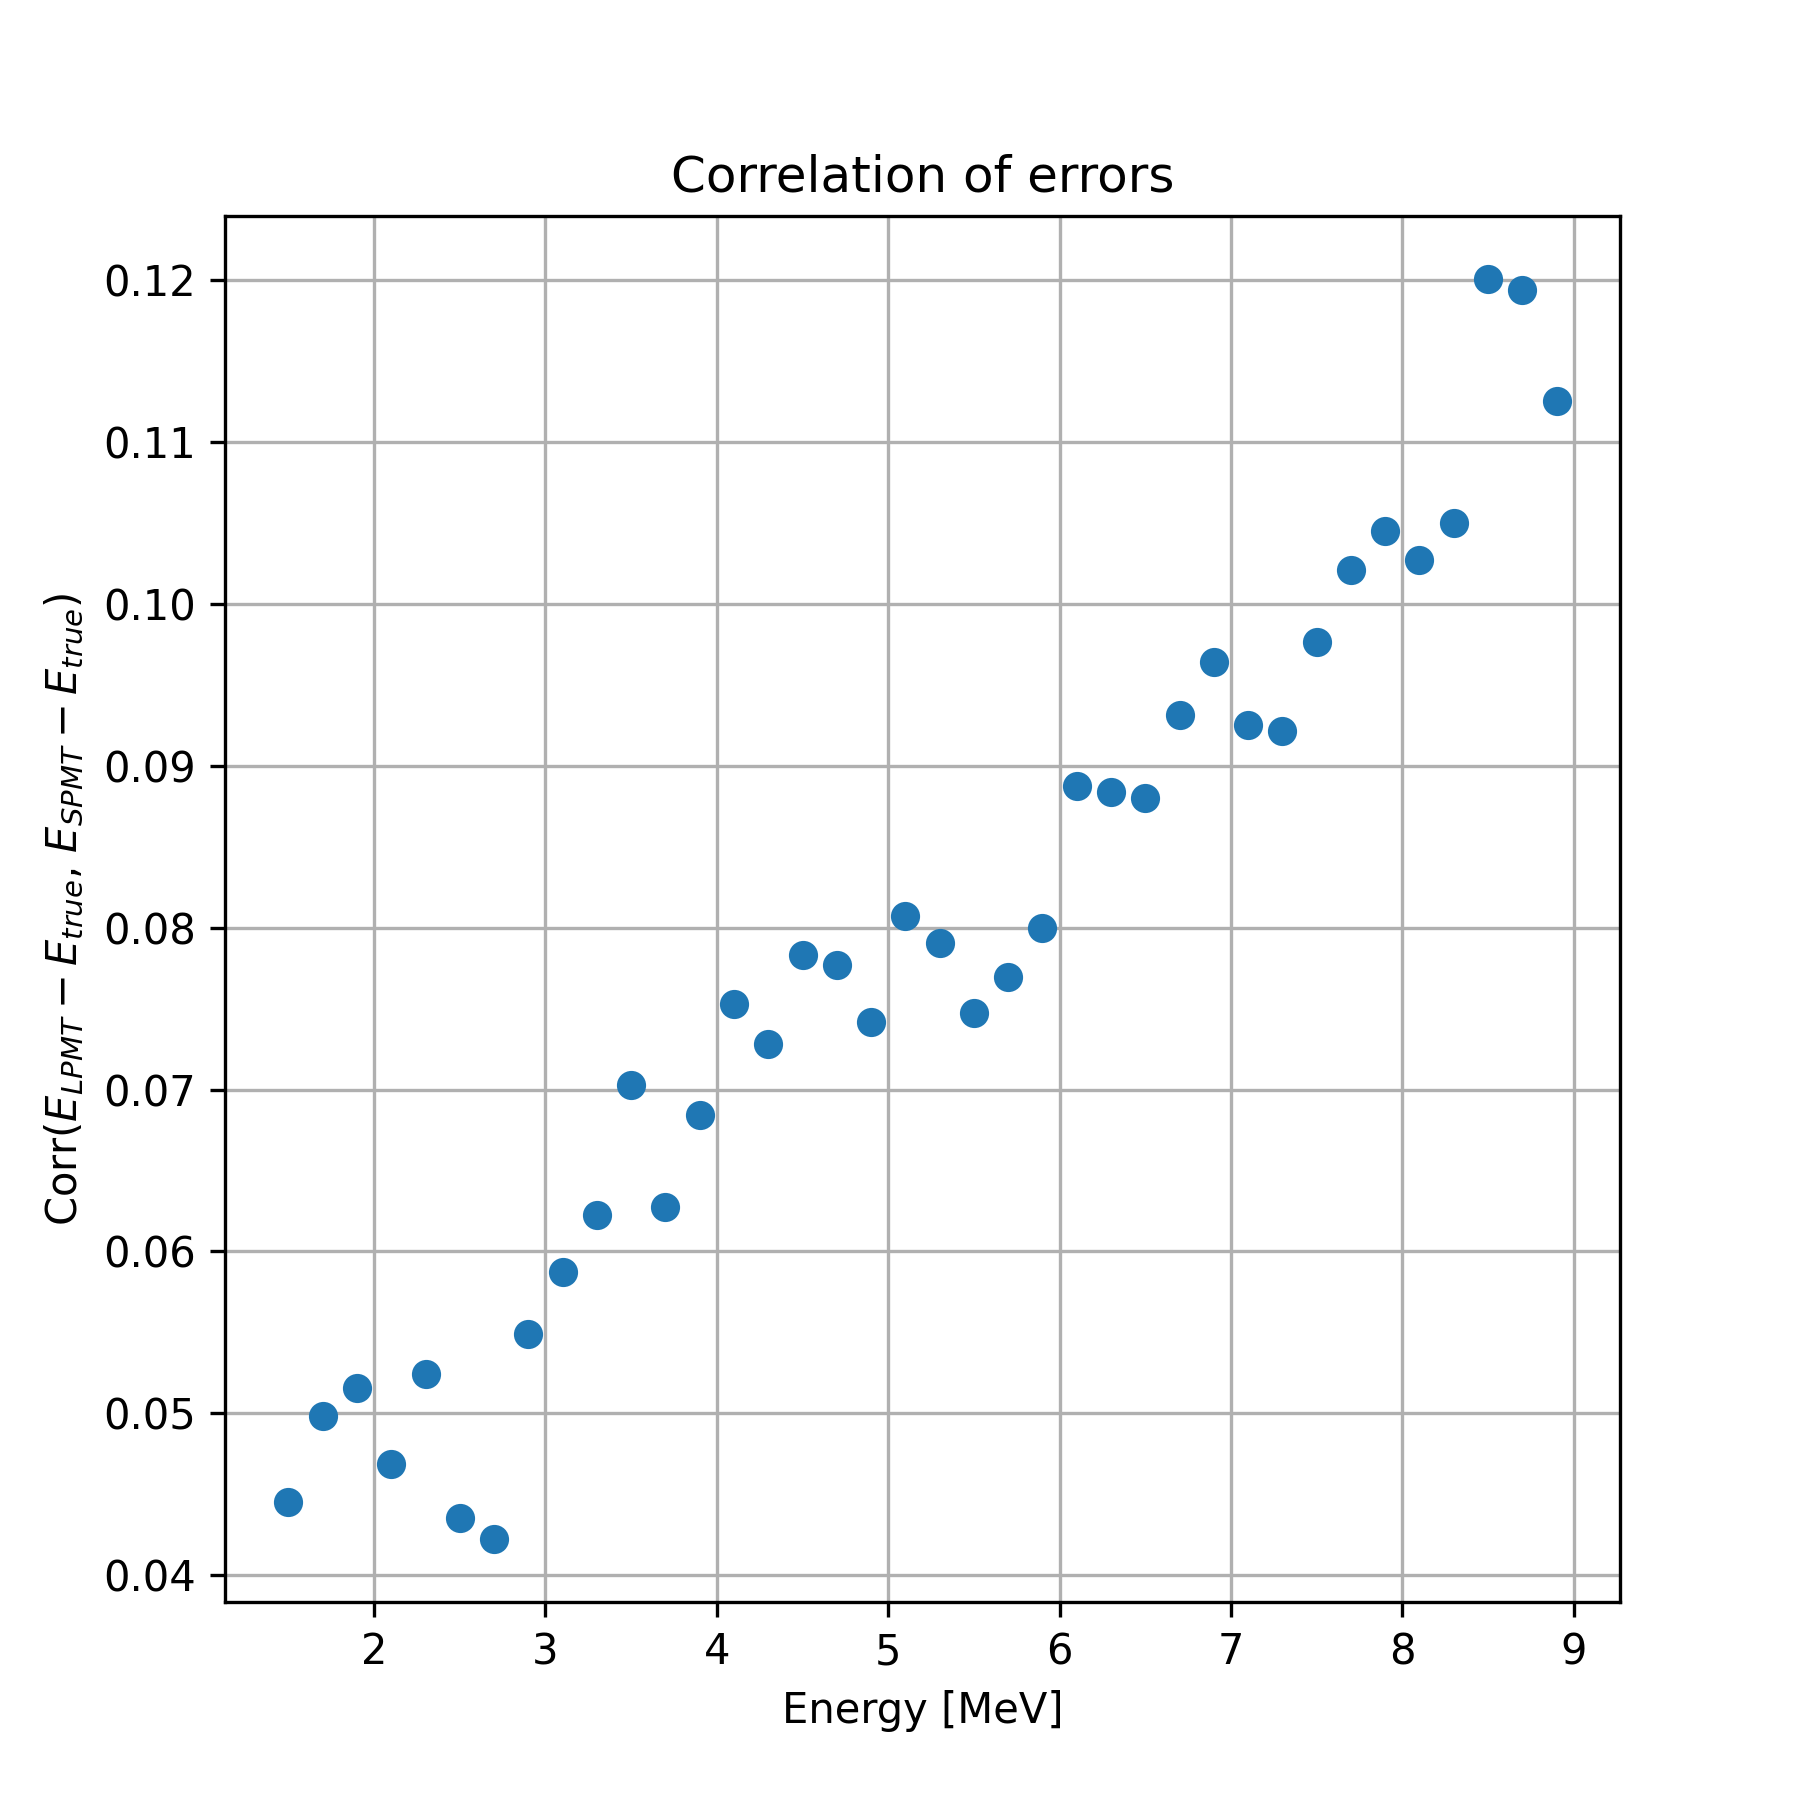
\includegraphics[width=\linewidth]{images/joint_fit/E_corr.png}
  \end{subfigure}
  \hfill
  \begin{subfigure}[t]{0.48\linewidth}
    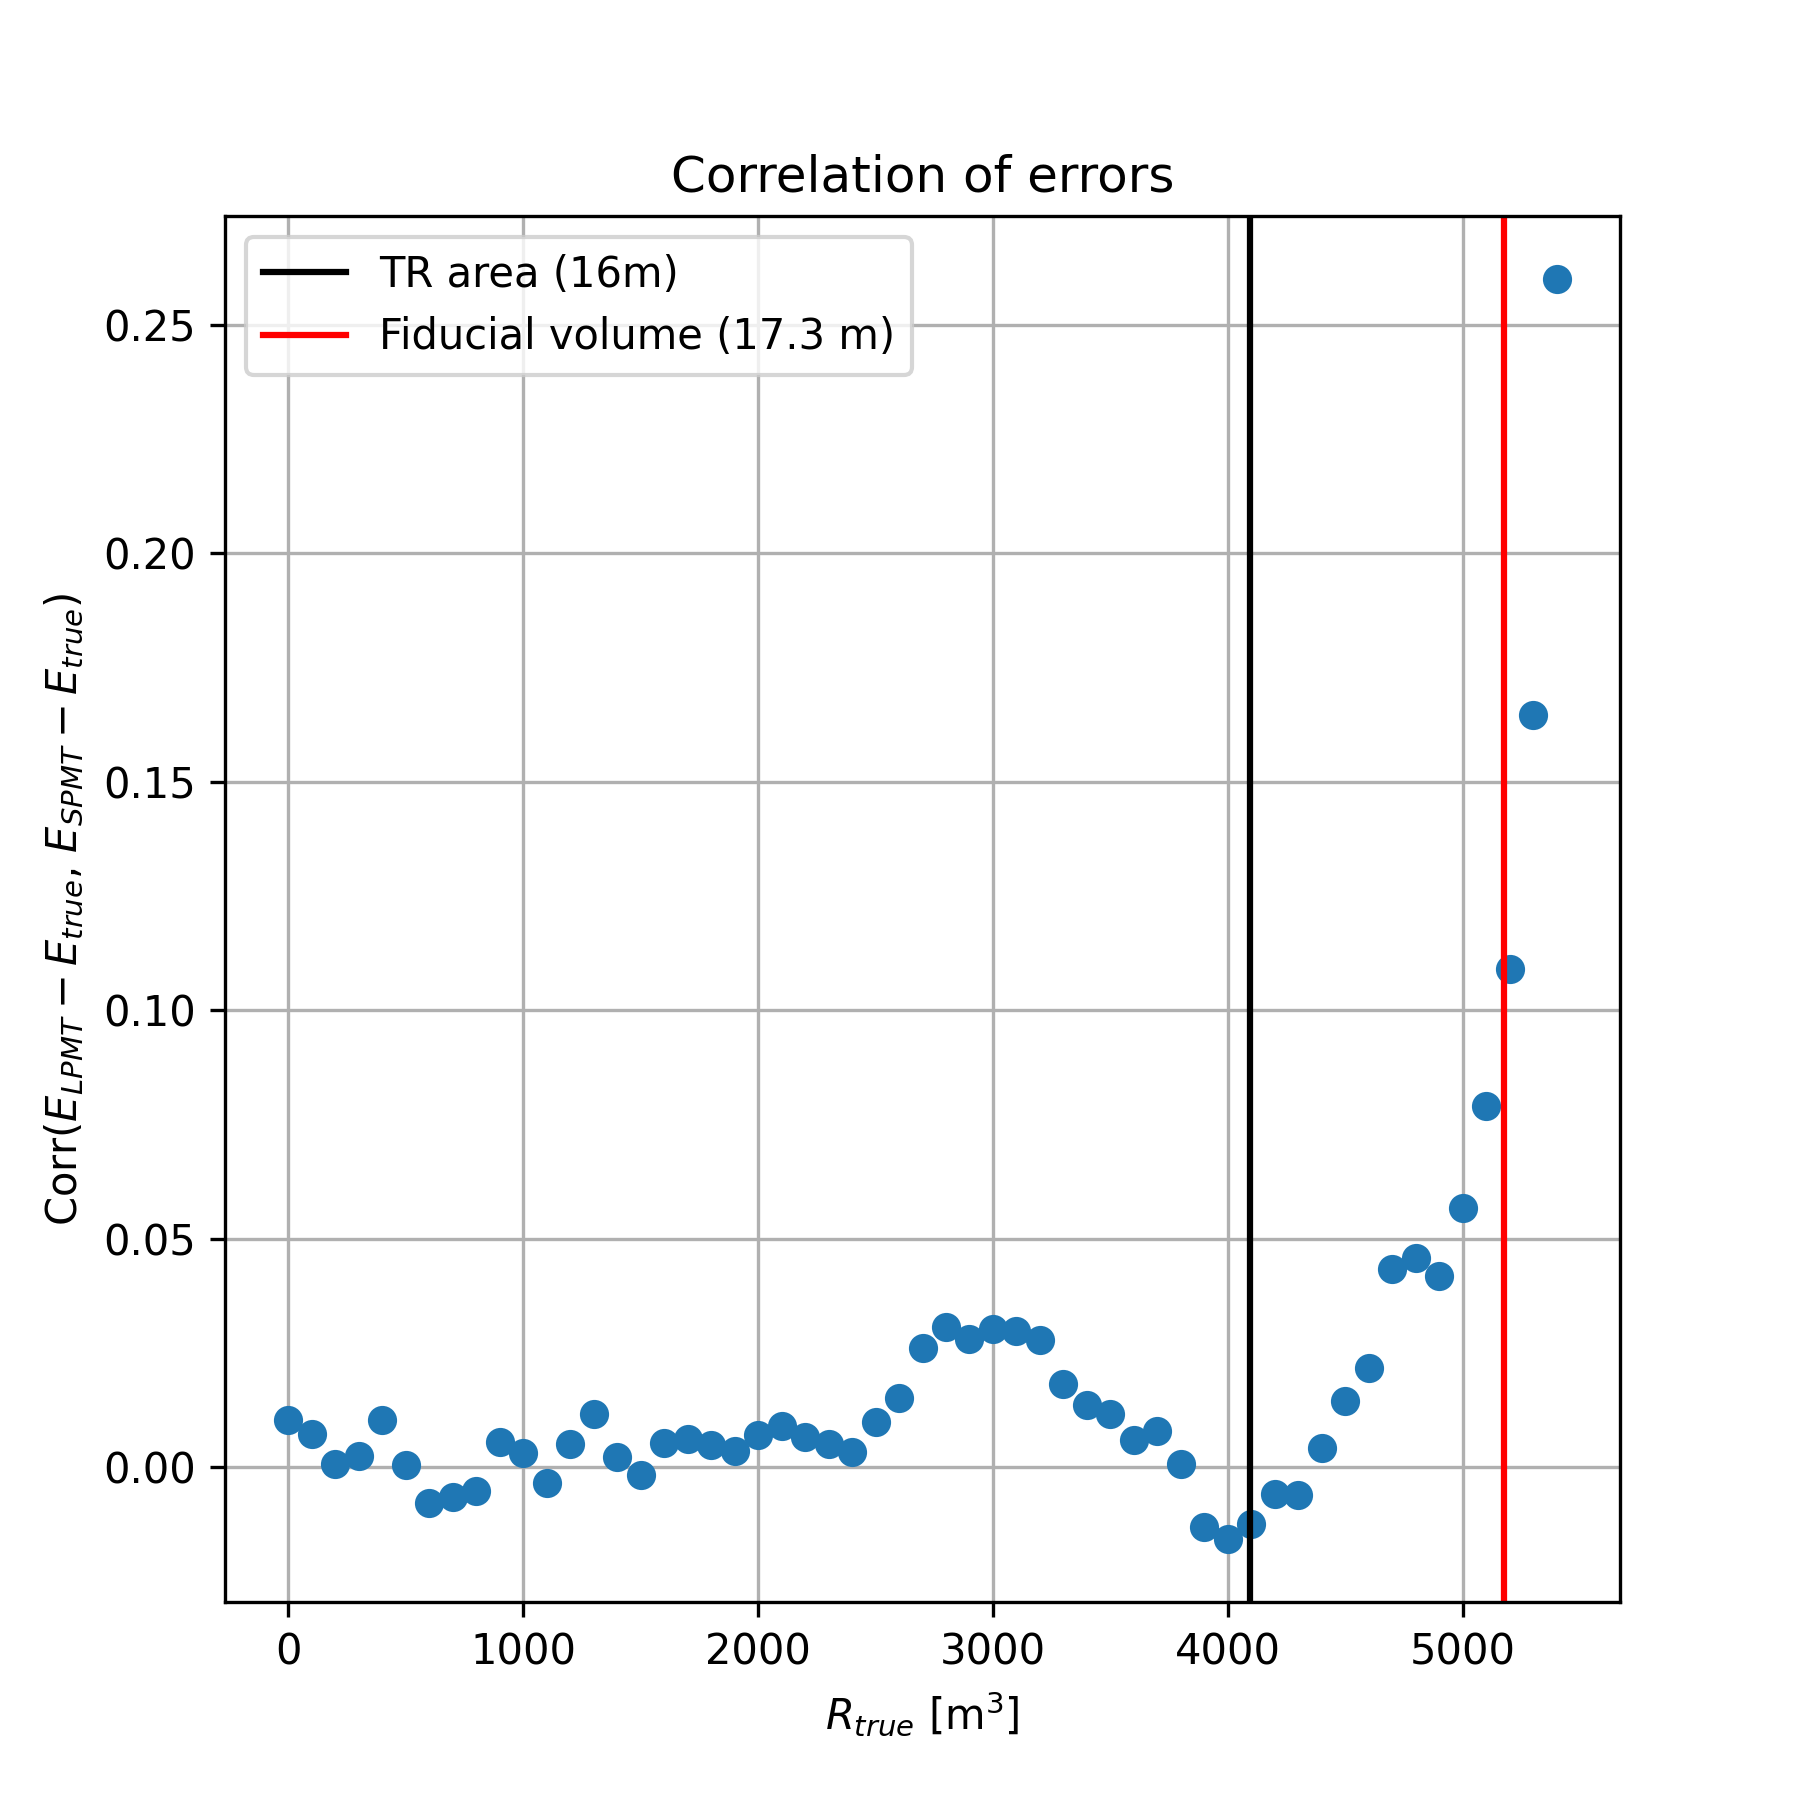
\includegraphics[width=\linewidth]{images/joint_fit/R_corr.png}
  \end{subfigure}
  \caption{Correlation on the reconstruction error between the LPMT and SPMT system as a function of \textbf{(On the left)} the energy, \textbf{(On the right)} the radius. The SPMT reconstruction comes from the NN presented in Chapter \ref{sec:jcnn} and the LPMT reconstruction comes from OMILREC presented in section \ref{sec:juno:reco}. To prevent effect due to the CNN bad reconstruction, we select the event with $1 < E_{dep} < 9$ MeV.}
  \label{fig:joint_fit:empirical_corr:E_a_R}
\end{figure}

We see correlation increase with respect to the energy which can be attributed to the signal over dark noise ratio. As more PMTs hits come from the signal, the reconstruction becomes more signal related. Regarding the $R^3$ distribution, we see almost no dependency until the total reflection area. After this point the correlation rises as the event are exposed to the optical effect of the total reflection area.

By looking at figure \ref{fig:joint_fit:empirical_corr:E_R}, we can see that the rising in correlation with respect to the energy is mostly due to the radius dependency.

\begin{figure}[ht]
  \centering
  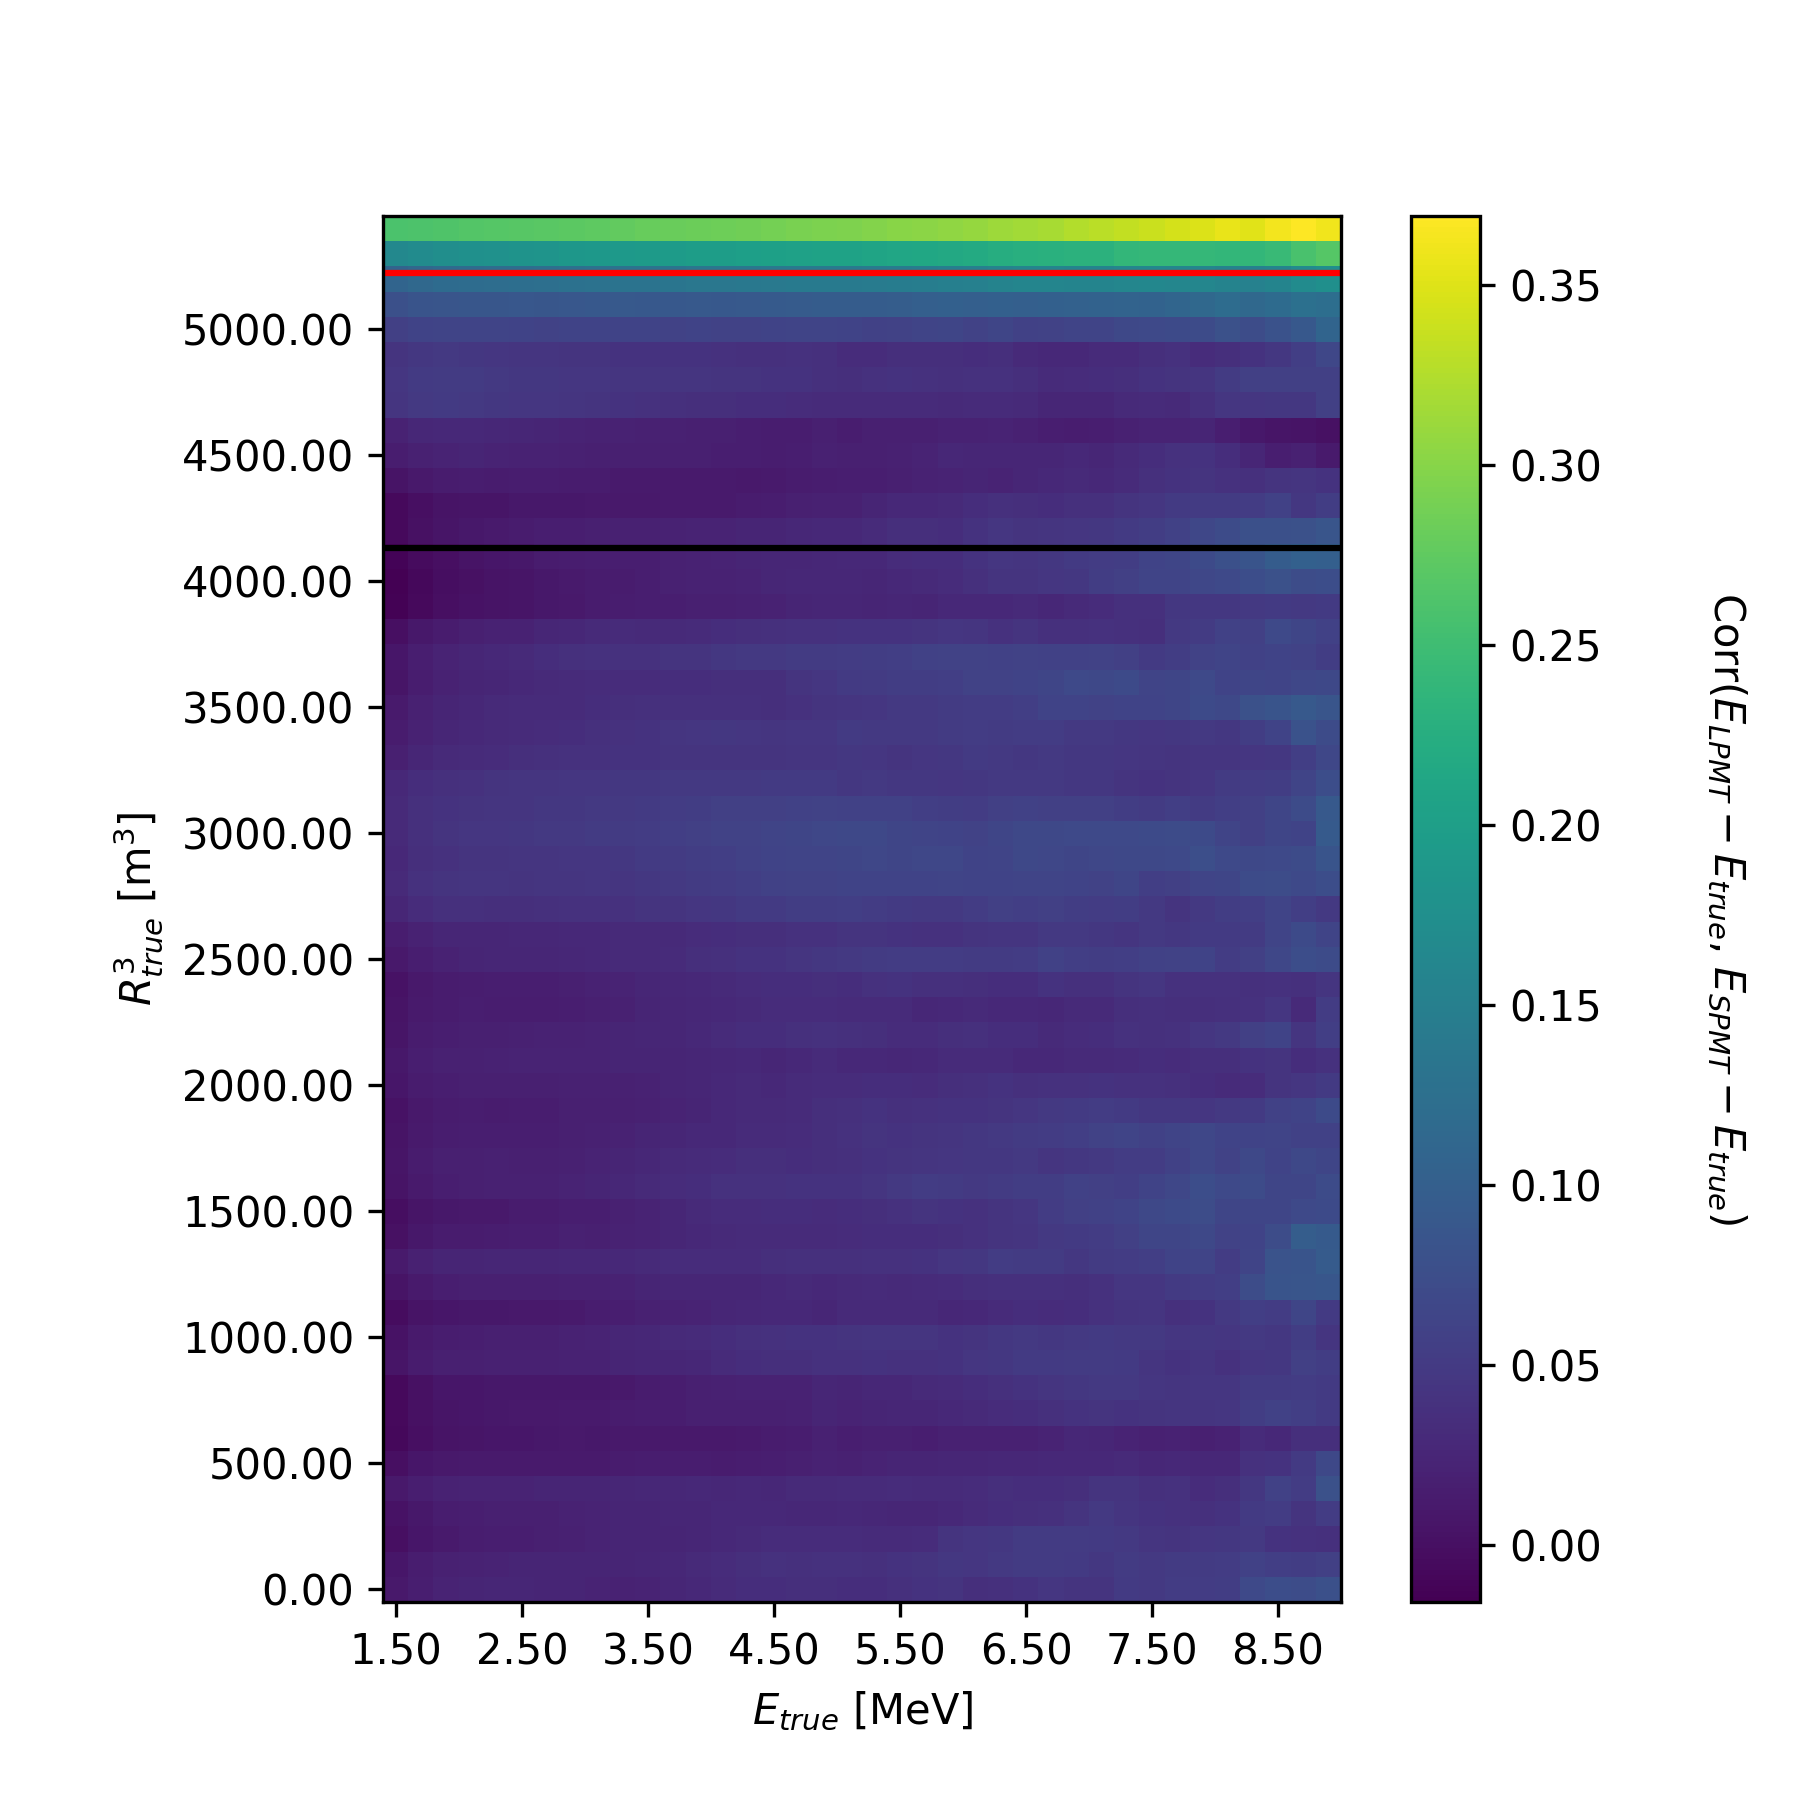
\includegraphics[height=6cm]{images/joint_fit/E_R_corr.png}
  \caption{Correlation on the reconstruction error between the LPMT and SPMT system as a function of  the energy and the radius. The SPMT reconstruction comes from the NN presented in Chapter \ref{sec:jcnn} and the LPMT reconstruction comes from OMILREC presented in section \ref{sec:juno:reco}. To prevent effect due to the CNN bad reconstruction, we select the event with $1 < E_{dep} < 9$ MeV.}
  \label{fig:joint_fit:empirical_corr:E_R}
\end{figure}

The exploitation of those correlations in the fit and the data production, without generating and reconstructing full spectra from SNIPER, is a bit more complicated. As seen in section \ref{sec:joint_fit:framework:ibd-gen}, we characterize the resolution of both systems by the ABC parameters. The correlation shown here take into account all of the ABC terms, as they are the complete correlation between the two systems, but the generation and the modeling this correlation needs to be very well understood as, as seen before, the mass ordering and parameters measurements are very sensitive to even small correlations.

We consider the binned approach that we used here, knowing that the CNN reconstruction was deemed efficient but flawed, to be insufficient for the complete study of those effects on the fit.

\subsection{Statistical tests}

In this part, I present the results of the statistical tests presented in section \ref{sec:joint_fit:approach}.

\subsubsection{Test $\chi^2_{spe}$}

The $\chi^2_{spe}$ is a chi-square representing the compatibility between the LPMT ans SPMT spectra under constraints of the correlation matrix between the two.
\begin{equation}
  \chi^2_{spe} = \bm{\Delta h} V_{spe} \bm{\Delta h}^T; ~ \bm{\Delta h} = \{ (h_0^L - h_0^S), ..., (h_n^L - h_n^S) \}
\end{equation}
where $h_i^L$ and $h_i^S$ are the contents of the $i$th bins of the LPMT and SPMT spectra. For details about the calculation of $V_{spe}$, see section \ref{sec:joint_fit:approach}.

The results for different exposures can be found in figure \ref{fig:joint_fit:chi2_spec}. To give an idea of the significance of this test, we provide the median p-value for each test $\alpha_{qnl} \neq 0$. As expected, the power of this test rises as the exposure does. We see significant discrimination at 6 years for $\alpha_{qnl} \geq 0.3 \%$ where the p-value for $\alpha_{qnl} = 3\%$ is $0.005 \pm 0.0022$.


\begin{figure}[th]
  \centering
  \begin{subfigure}[t]{0.48\linewidth}
    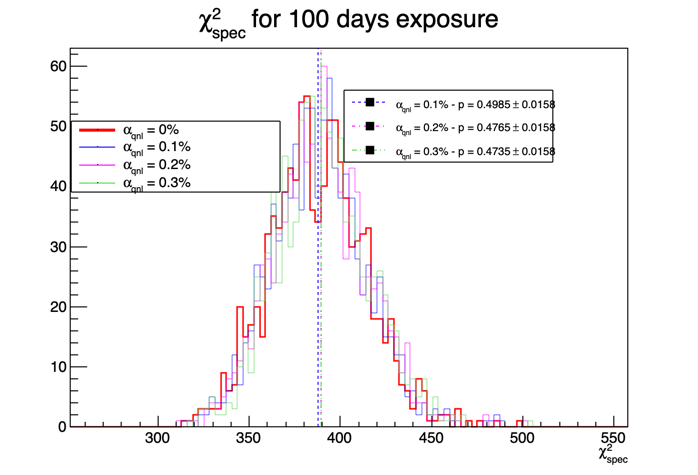
\includegraphics[width=\linewidth]{images/joint_fit/stat_tests/chi2_spec_100d.png}
  \end{subfigure}
  \begin{subfigure}[t]{0.48\linewidth}
    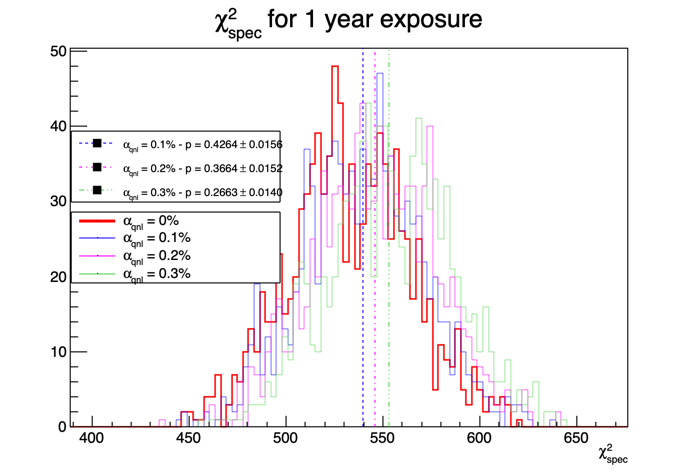
\includegraphics[width=\linewidth]{images/joint_fit/stat_tests/chi2_spec_1y.png}
  \end{subfigure}


  \begin{subfigure}[t]{0.48\linewidth}
    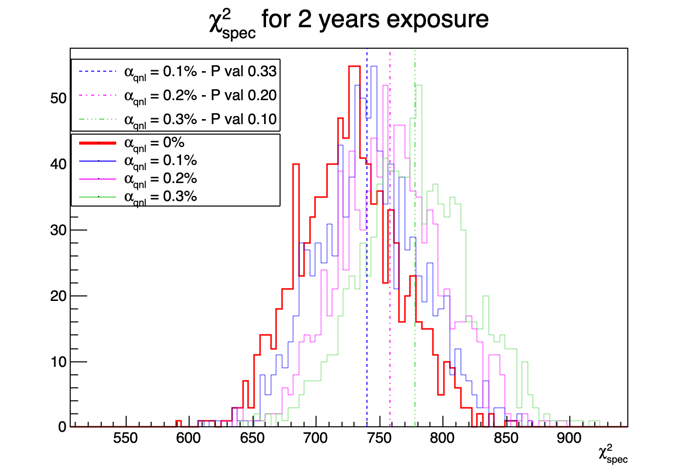
\includegraphics[width=\linewidth]{images/joint_fit/stat_tests/chi2_spec_2y.png}
  \end{subfigure}
  \begin{subfigure}[t]{0.48\linewidth}
    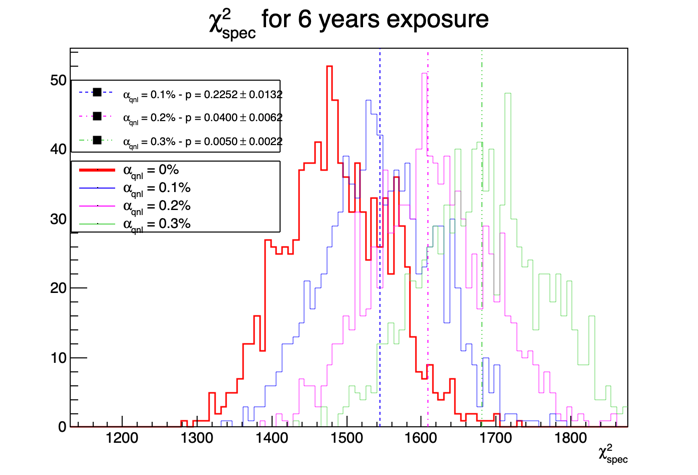
\includegraphics[width=\linewidth]{images/joint_fit/stat_tests/chi2_spec_6y.png}
  \end{subfigure}
  \caption{Distribution of the $\chi^2_{spe}$ for 1000 toys for different exposure. The dashed line represent the median of the distribution and the p-value are the percentage of the $\alpha_{qnl} = 0$ distribution that are greater than those medians.}
  \label{fig:joint_fit:chi2_spec}
\end{figure}

This test relies solely on the estimated covariance matrix between the two spectra, requiring no fitting. As a result, it is a very lightweight test that can still provide valuable indications of potential unknown distortions between the two spectra.

\subsubsection{Test $\chi^2_{ind}$}

The $\chi^2_{ind}$ is the chi-square that represent the agreement between the measured oscillation parameters $\theta_{12}$ and $\Delta m^2_{21}$. This test is defined as
\begin{equation}
  \chi^2_{ind} = \bm{\Delta \lambda} V_{ind} \bm{\Delta \lambda}^T; ~ \bm{\Delta \lambda} = \{\theta_{12}^L - \theta_{12}^S, (\Delta m^2_{21})^L - (\Delta m^2_{21})^S\}
\end{equation}
where $\theta^L_{12}$ and $(\Delta m^2_{21})^L$ are the oscillation parameters measured by the LPMT system. Same for $\theta_{12}^S$ and $(\Delta m^2_{21})^S$ for the SPMT system. We use $V_{ind}$ computed for $\alpha_{qnl} = 0$. For more details about the calculation of $V_{ind}$ see section \ref{sec:joint_fit:approach}.

The results are presented in figure \ref{fig:joint_fit:chi2_ind}. This test does not require any joint fit or covariance matrix estimation between the two spectrum, it just need the estimated covariance matrix between the four parameters. We see that the p-value are much less significant than the other tests, this is because this test possess much less information about the relation between the LPMT and SPMT systems.

\begin{figure}[th]
  \centering
  \begin{subfigure}[t]{0.48\linewidth}
    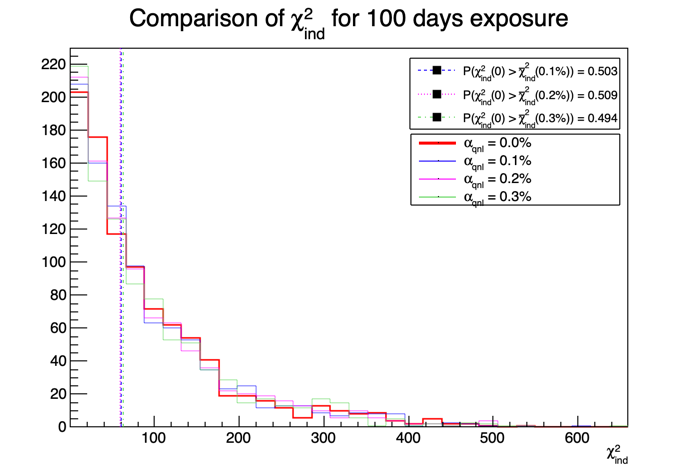
\includegraphics[width=\linewidth]{images/joint_fit/stat_tests/chi2_ind_100d.png}
  \end{subfigure}
  \begin{subfigure}[t]{0.48\linewidth}
    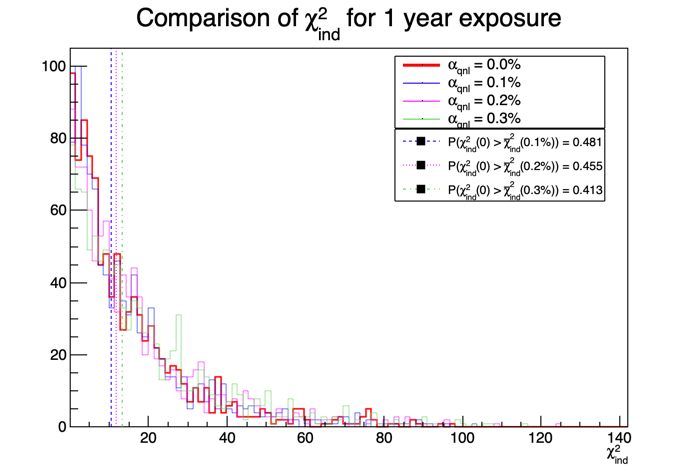
\includegraphics[width=\linewidth]{images/joint_fit/stat_tests/chi2_ind_1y.png}
  \end{subfigure}


  \begin{subfigure}[t]{0.48\linewidth}
    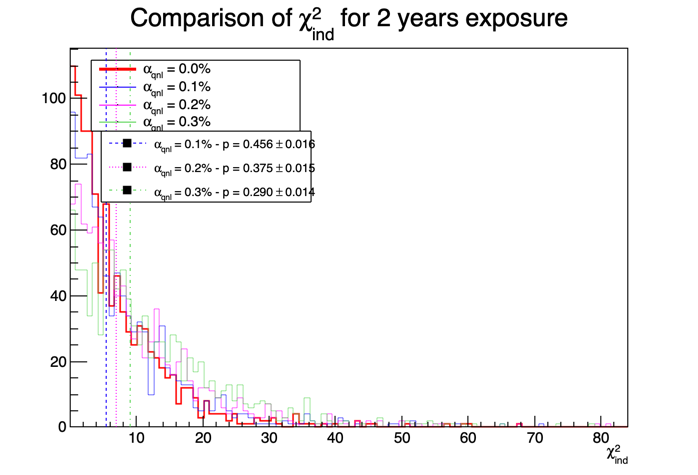
\includegraphics[width=\linewidth]{images/joint_fit/stat_tests/chi2_ind_2y.png}
  \end{subfigure}
  \begin{subfigure}[t]{0.48\linewidth}
    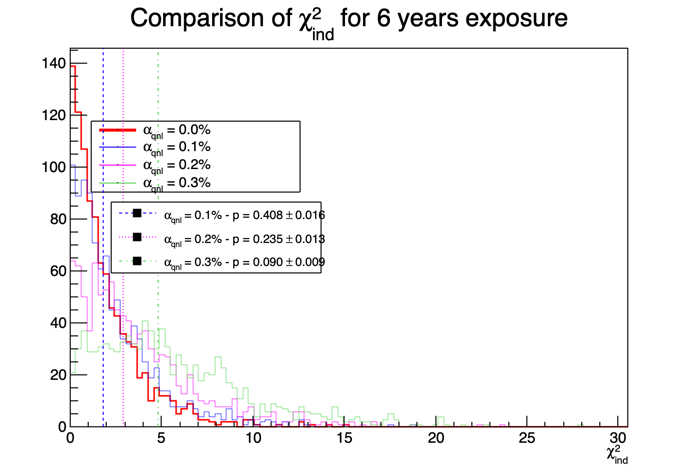
\includegraphics[width=\linewidth]{images/joint_fit/stat_tests/chi2_ind_6y.png}
  \end{subfigure}
  \caption{Distribution of the $\chi^2_{ind}$ for 1000 toys for different exposures. The dashed lines represent the median of the distributions and the p-value are the percentage of the $\alpha_{qnl} = 0$ distribution that are greater than those medians.}
  \label{fig:joint_fit:chi2_ind}
\end{figure}

This test is the most straightforward as it require only the fit of the two spectra and the estimation of the parameters covariances, but is also the less powerful with a p value for $\alpha_{qnl} = 0.3\%$ of $0.09 \pm 0.009$.

\subsubsection{$\delta$ parameters significance}

This test involves observing the values of the $\delta$ parameters in the Delta Joint fit and comparing them tho their dispersion in the case where $\alpha_{qnl} = 0$. The results are shown in figures \ref{fig:joint_fit:chi2_delta} and \ref{fig:joint_fit:chi2_delta_m}.

\begin{figure}[th]
  \centering
  \begin{subfigure}[t]{0.48\linewidth}
    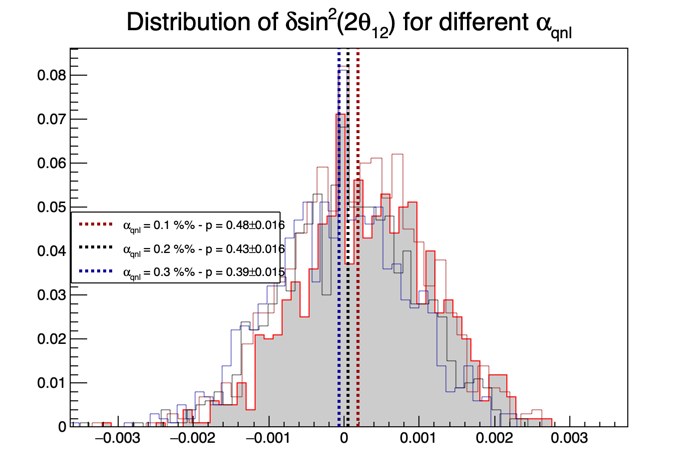
\includegraphics[width=\linewidth]{images/joint_fit/stat_tests/chi2_delta_100d.png}
    \caption{100 days exposure}
  \end{subfigure}
  \begin{subfigure}[t]{0.48\linewidth}
    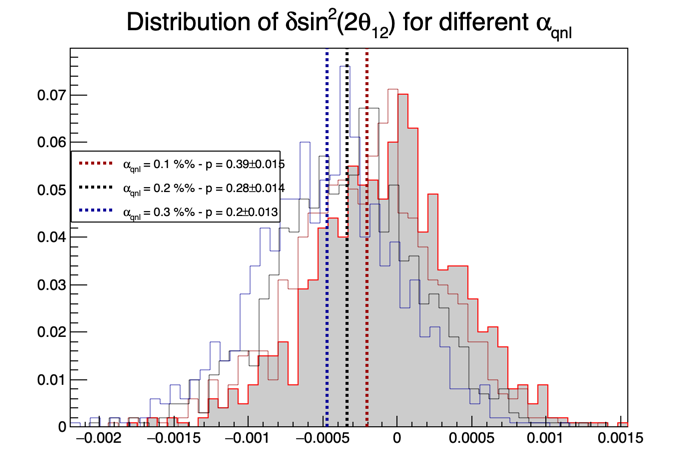
\includegraphics[width=\linewidth]{images/joint_fit/stat_tests/chi2_delta_1y.png}
    \caption{1 year exposure}
  \end{subfigure}


  \begin{subfigure}[t]{0.48\linewidth}
    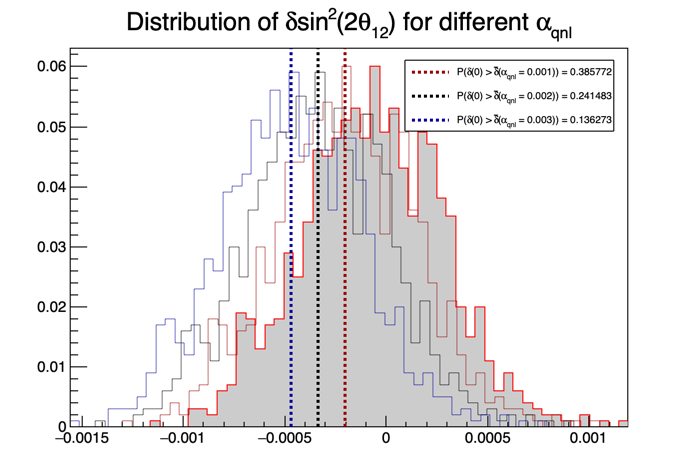
\includegraphics[width=\linewidth]{images/joint_fit/stat_tests/chi2_delta_2y.png}
    \caption{2 years exposure}
  \end{subfigure}
  \begin{subfigure}[t]{0.48\linewidth}
    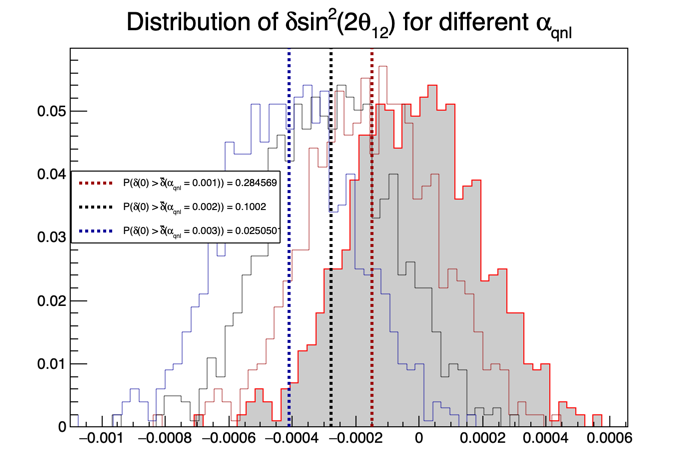
\includegraphics[width=\linewidth]{images/joint_fit/stat_tests/chi2_delta_6y.png}
    \caption{6 years exposure}
  \end{subfigure}
  \caption{Distribution of the $\delta \sin^2(2\theta_{12})$ for 1000 toys for different exposure. The dashed line represent the median of the distribution and the p-value are the percentage of the $\alpha_{qnl} = 0$ distribution that are greater than those medians.}
  \label{fig:joint_fit:chi2_delta}
\end{figure}


\begin{figure}[th]
  \centering
  \begin{subfigure}[t]{0.48\linewidth}
    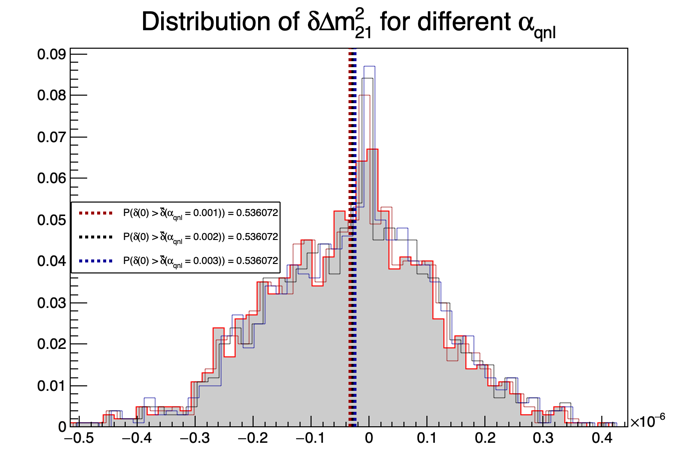
\includegraphics[width=\linewidth]{images/joint_fit/stat_tests/chi2_delta_m_100d.png}
    \caption{100 days exposure}
  \end{subfigure}
  \begin{subfigure}[t]{0.48\linewidth}
    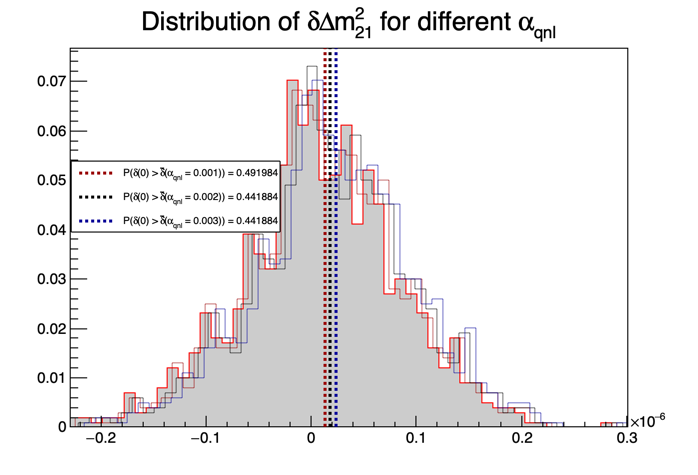
\includegraphics[width=\linewidth]{images/joint_fit/stat_tests/chi2_delta_m_1y.png}
    \caption{1 year exposure}
  \end{subfigure}


  \begin{subfigure}[t]{0.48\linewidth}
    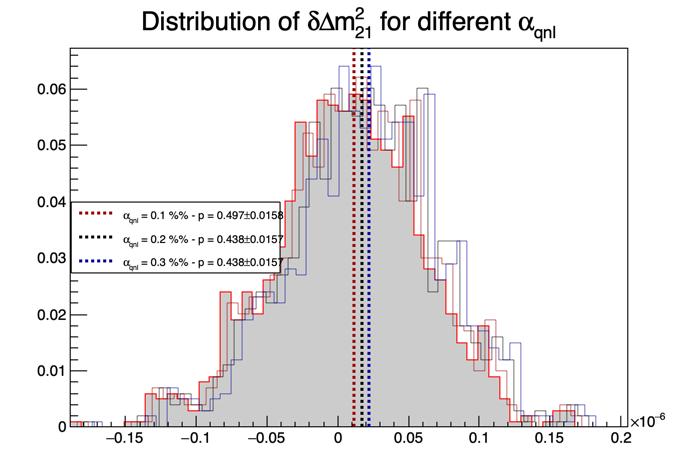
\includegraphics[width=\linewidth]{images/joint_fit/stat_tests/chi2_delta_m_2y.png}
    \caption{2 years exposure}
  \end{subfigure}
  \begin{subfigure}[t]{0.48\linewidth}
    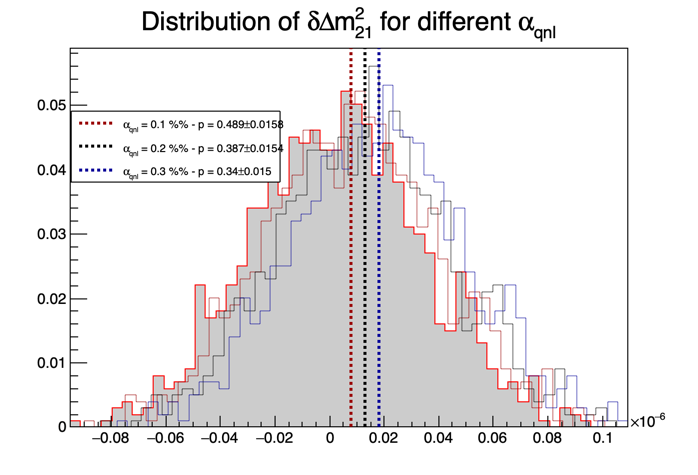
\includegraphics[width=\linewidth]{images/joint_fit/stat_tests/chi2_delta_m_6y.png}
    \caption{6 years exposure}
  \end{subfigure}
  \caption{Distribution of the $\delta \Delta m^2_{21}$ for 1000 toys for different exposure. The dashed line represent the median of the distribution and the p-value are the percentage of the $\alpha_{qnl} = 0$ distribution that are greater than those medians.}
  \label{fig:joint_fit:chi2_delta_m}
\end{figure}

We can see that the $\delta \Delta m^2_{21}$ has a very small discriminative power (figure \ref{fig:joint_fit:chi2_delta_m}) even at 6 years exposure with a p-value of $0.34 \pm 0.01$ for $\alpha_{qnl} = 0.3\%$. On the other hand $\delta \theta_{12}$ (figure \ref{fig:joint_fit:chi2_delta}) has much more discriminative power with a p-value for $\alpha_{qnl} = 0.3\%$ of $0.025 \pm 0.005$. This test with a single joint fit seems to be still less powerful than the $\chi^2_{spe}$. This can be explained as this method only get information through the oscillation parameters $\theta_{12}$ and $\Delta m^2_{21}$ missing potential informations contained in $\Delta m^2_{31}$.

\subsubsection{Hypothesis test}

In this last test we consider the two fit Standard Joint and Delta Joint as two hypothesis. The first one, Standard Joint, is the $H_0$ hypothesis: we do not need supplementary parameters to describe the energy spectrum. The second one, Delta Joint, is the $H_1$ hypothesis: we do need those supplementary $\delta$ parameters to, if not correctly, approach the energy spectrum. If the $\delta$ parameter are unnecessary the $\chi^2_{H_0}$ should be close to $\chi^2_{H_1}$. On the other hand, if one spectrum is distorted, then those parameters are relevant and $\chi^2_{H_1} < \chi^2_{H_0}$. For this test we thus observe the $\chi^2_{H_0} - \chi^2_{H_1}$ distributions for different exposures and $\alpha_{qnl}$. The results are presented in figure \ref{fig:joint_fit:chi2_H}.

\begin{figure}[th]
  \centering
  \begin{subfigure}[t]{0.48\linewidth}
    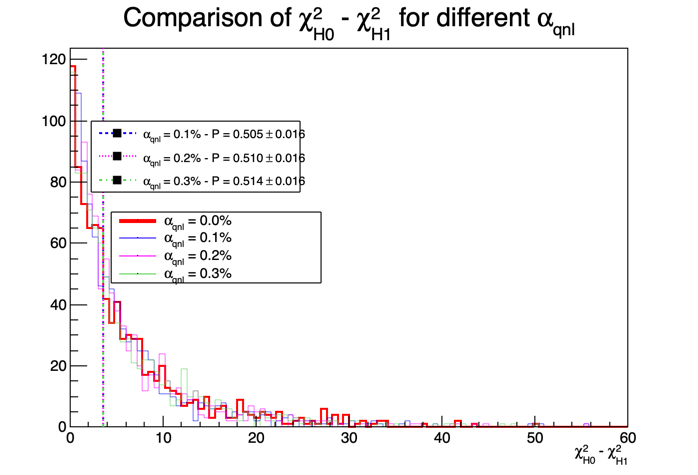
\includegraphics[width=\linewidth]{images/joint_fit/stat_tests/chi2_H_100d.png}
    \caption{100 days exposure}
  \end{subfigure}
  \begin{subfigure}[t]{0.48\linewidth}
    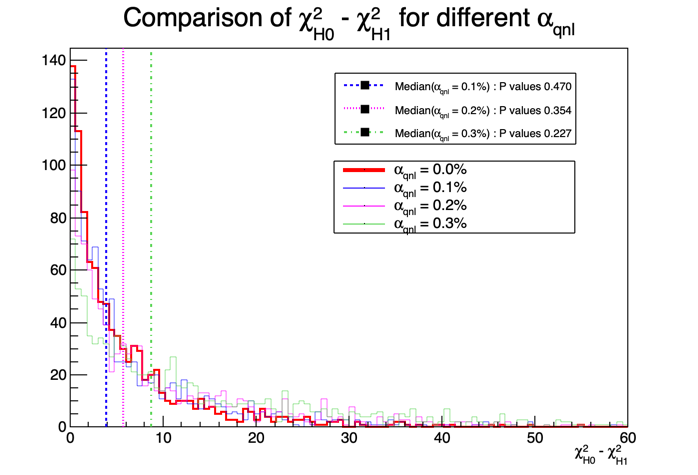
\includegraphics[width=\linewidth]{images/joint_fit/stat_tests/chi2_H_1y.png}
    \caption{1 year exposure}
  \end{subfigure}


  \begin{subfigure}[t]{0.48\linewidth}
    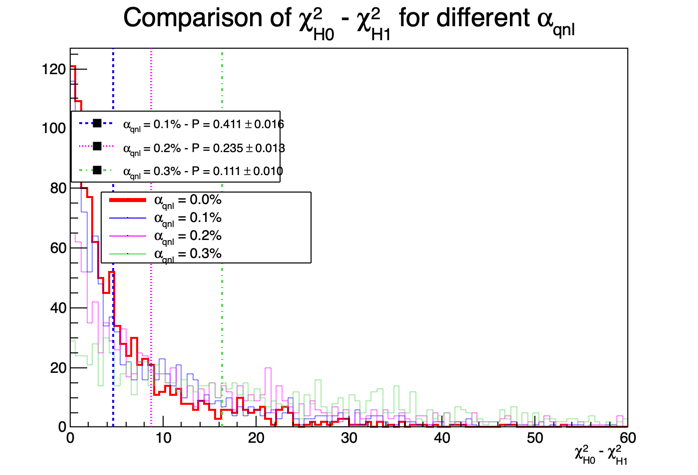
\includegraphics[width=\linewidth]{images/joint_fit/stat_tests/chi2_H_2y.png}
    \caption{2 years exposure}
  \end{subfigure}
  \begin{subfigure}[t]{0.48\linewidth}
    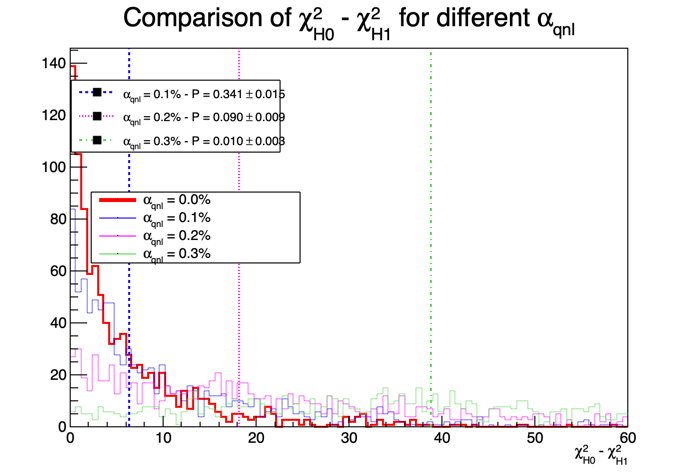
\includegraphics[width=\linewidth]{images/joint_fit/stat_tests/chi2_H_6y.png}
    \caption{6 years exposure}
  \end{subfigure}
  \caption{Distribution of $\chi^2_{H_0} - \chi^2_{H_1}$ for 1000 toys for different exposure. The dashed line represent the median of the distribution and the p-value are the percentage of the $\alpha_{qnl} = 0$ distribution that are greater than those medians.}
  \label{fig:joint_fit:chi2_H}
\end{figure}

This test is the most complex, requiring two fit and the covariance matrix between the LPMT and SPMT spectra. The results are good, close to the $\chi^2_{spe}$, one with a p-value at 6 years for $\alpha_{qnl} = 0.3\%$ of $0.01 \pm 0.003$.

As explained in section \ref{sec:joint_fit:data_gen}, the spectra used for the fit are cut at 335 bins / 7.5 MeV to prevent instability, while in $\chi^2_{spe}$ we use full 410 bins spectra. The $\chi^2_{spe}$ thus has more informations that the hypothesis test leading to this difference in power.

% Montre chi^2_{spe} 335 ?

%
%   (c) Résultats fit séparés
%
%
%   (d) Résultats fits joints
%
%   (e) Résultats avec corrélations reco_spmt vs. reco_lmpt mieux prises en compte
%

\section{Conclusion and perspectives}
\label{sec:joint_fit:conclusion}
% Vll) Discussions, perspectives

In this chapter, we present the development of a fit framework that allows us to fit multiple spectra simultaneously. We also introduce a set of tools that enable us to detect potential distortions in one of the two spectra. As an illustration of the capability of these tools, we use supplementary event-wise non-linearity and compare it to the potential residual event-wise non-linearity after calibration. Our results show that after 6 years of data collection, we can reject the median residual distortion with a p-value of 0.5\% under the conditions outlined in this chapter.

Additionally, this study is preliminary, as the background was neglected in the distortion test, and no systematic uncertainties were considered. The supplementary non-linearity was introduced event-wise but should be applied channel-wise to account for the detector's non-uniformity. The correlation matrix between the LPMT and SPMT spectra should also be further analyzed, as indicated by the discrepancies between the theoretical and empirical correlation matrices. We should also further investigate the effect of non-uniformity on the correlation matrix.

\end{document}
